\documentclass[10pt,a4paper]{article}

% ==================== PACKAGES ====================
\usepackage[utf8]{inputenc}
\usepackage[T1]{fontenc}
\usepackage{lmodern}
\usepackage[a4paper, margin=2.1cm, headheight=14pt]{geometry}
\usepackage{amsmath, amssymb}
\usepackage{array}
\usepackage{tabularx}
\usepackage{multirow}
\usepackage{float}
\usepackage{graphicx}
\usepackage{caption}
\usepackage{subcaption}
\usepackage{fancyhdr}
\usepackage{titlesec}
\usepackage{enumitem}
\usepackage{multicol}
\usepackage{xcolor}
\usepackage{colortbl}
\usepackage{microtype}
\usepackage{ragged2e}
\usepackage[hidelinks]{hyperref}
\usepackage{tikz}
\usepackage{pgfplots}

\usetikzlibrary{arrows.meta, positioning, shapes.geometric, patterns, calc}
\usepgfplotslibrary{groupplots}
\pgfplotsset{compat=1.18}
\emergencystretch=1.5em

% ==================== STRICT PURE BLACK & WHITE STYLING ====================
\definecolor{barhand}{gray}{0.20}
\definecolor{barlk}{gray}{0.65}

% Pure white table headers (zero background fill)
\newcommand{\hdrrow}{}

% Crisp bordered table spacing
\renewcommand{\arraystretch}{1.28}
\setlength{\tabcolsep}{5pt}
\setlength{\arrayrulewidth}{0.55pt}

% Paragraph & list spacing
\setlength{\parindent}{0pt}
\setlength{\parskip}{5.5pt}
\setlist[itemize]{nosep, leftmargin=1.4em, itemsep=2.5pt}

% Section formatting (pure black)
\titleformat{\section}{\large\bfseries\color{black}}{\thesection}{0.75em}{}
\titleformat{\subsection}{\normalsize\bfseries\color{black}}{\thesubsection}{0.75em}{}
\titlespacing*{\section}{0pt}{11pt}{4pt}
\titlespacing*{\subsection}{0pt}{8pt}{3pt}

% Captions (fully justified)
\captionsetup{font=small, labelfont=bf, justification=justified, singlelinecheck=false, skip=5pt}

% Running headers & footers (pure black)
\pagestyle{fancy}
\fancyhf{}
\fancyhead[L]{\small\color{black} Continuous Ethyl Acetate Production}
\fancyhead[R]{\small\color{black} K. Bazrafkan Esfahani}
\fancyfoot[C]{\small\color{black} \thepage}
\renewcommand{\headrulewidth}{0.6pt}
\renewcommand{\footrulewidth}{0pt}

% Helper column types (Y justified for prose columns; J justified fixed-width)
\newcolumntype{L}[1]{>{\centering\arraybackslash}m{#1}}
\newcolumntype{J}[1]{>{\centering\arraybackslash}m{#1}}
\newcolumntype{R}[1]{>{\centering\arraybackslash}m{#1}}
\newcolumntype{C}[1]{>{\centering\arraybackslash}m{#1}}
\newcolumntype{Y}{>{\centering\arraybackslash}X}
\newcolumntype{Z}{>{\centering\arraybackslash}X}

% Justified table footnote macro
\newcommand{\tabnote}[1]{\par\vspace{2pt}\begin{minipage}{\textwidth}\justifying\footnotesize #1\end{minipage}}

\begin{document}

% ==================== PAGE 1: OFFICIAL PORTFOLIO COVER ====================
\begin{titlepage}
\thispagestyle{empty}
\centering
\vspace*{2.4cm}

{\LARGE\bfseries Continuous Ethyl Acetate Production\par}
\vspace{0.85cm}
{\large\bfseries DWSIM Simulation with NRTL, Independent Verification\\and Thermodynamic Sensitivity Study\par}
\vspace{3.6cm}

{\large\bfseries Technical Portfolio Project\par}
\vspace{3.6cm}

{\large\bfseries Kian Bazrafkan Esfahani\par}
\vspace{0.45cm}
{\normalsize Chemical Engineering, The University of Manchester\par}
\vspace{0.45cm}
{\normalsize November 2026\par}

\vfill
\end{titlepage}

\setcounter{page}{2}

% ==================== PAGE 2: EXECUTIVE SUMMARY ====================
\section*{Executive Summary}
\addcontentsline{toc}{section}{Executive Summary}

\subsection*{Project Objective}
This report presents the design, simulation and independent verification of a small continuous esterification plant producing 1,000~kg/day (41.67~kg/h, or 330~t/year over 330 operating days) of ethyl acetate from ethanol and acetic acid over Amberlyst~35 resin. The flowsheet was built and solved in DWSIM~10.0 using the NRTL activity-coefficient model, a conversion reactor at 65\% single-pass conversion, component separators and a closed recycle loop, and cross-checked against an independent Python model that solves the same mass, energy, equilibrium and kinetic balances in closed form.

\subsection*{Simulation Traps Exposed by Independent Verification}
Testing DWSIM's default settings against physical expectations revealed three pitfalls that a converged flowsheet hides:
\begin{itemize}
  \item \textbf{False recycle convergence (snowball effect):} Because acetic acid sets the reaction extent, perturbations in excess ethanol circulate with a numerical loop gain of 0.990 (amplification factor~99), even though total ethanol makes only $\sim$3 physical reactor passes on average due to 32.5\% per-pass reaction consumption. A Python reconstruction of DWSIM's default direct-substitution procedure (0.01~kg/s tolerance from an empty tear stream) predicts false convergence after two iterations at only 41\% of the true recycle flow (25.4~kg/h vs.\ 62.62~kg/h), leaving EtOH:AA = 0.99 where 65\% exceeds the 58\% equilibrium estimate. Tightening the tolerance to $1 \times 10^{-8}$~kg/s resolves closure within $3.5 \times 10^{-5}$~kg/h (0.00007\% of fresh feed).
  \item \textbf{Enthalpy-method sensitivity:} DWSIM's default Lee--Kesler enthalpy option predicts heater (E2) and cooler (E4) duties 16\% and 19\% above the independent ideal-liquid NIST/DIPPR benchmark, alongside mixer warming (+4.9~K) and non-zero separator duties (0.28 and 0.19~kW). Switching to Liquid $C_p$ + Enthalpy of Vaporization brings E2 and E4 within 0.11\% and 0.03\% of that ideal-liquid benchmark (full physical accuracy still requires excess-enthalpy validation) and eliminates those artefacts, while raising reactor duty (E3) to 2.43~kW vs.\ 0.68~kW---numerically explained by a 1.75~kW ideal-gas reaction-enthalpy reference offset.
  \item \textbf{Thermodynamic database gaps:} DWSIM's NRTL database holds four of the six binary pairs and estimates the two acetic-acid pairs from UNIFAC. While literature azeotrope temperatures agree within 0.3~K, the ternary azeotrope ester mole fraction differs by 0.087 (0.666 vs.\ 0.579), a spurious acetic acid--water azeotrope appears, and the ethyl acetate--water miscibility gap is far too narrow for decanter design.
\end{itemize}

\subsection*{Verified Design \& Engineering Outcomes}
\begin{itemize}
  \item \textbf{Material balance \& product quality:} Both solved DWSIM runs agree with the closed-form Python hand calculation within 0.009\% for every component in every stream and pass all twelve acceptance checks, producing 41.68~kg/h of product at 99.96~wt\% ethyl acetate (94.9\% overall acetic acid conversion) within the composition limits of a commercial sales specification.
  \item \textbf{Reactor sizing \& heat integration:} Operating at a 2.00~mol/mol EtOH:AA reactor-inlet ratio keeps 65\% conversion below model-dependent equilibrium estimates of 73.5--81.2\%. Kinetic sizing with Amberlyst~35 requires 15.4~kg of catalyst in a plug-flow bed (against 48.9~kg in a CSTR), giving a $0.20\text{ m} \times 1.0\text{ m}$ design bed (25.1~kg). Feed--effluent heat exchange recovers 2.32~kW, cutting preheater duty by 73\% and cooler duty by 82\%.
\end{itemize}

\subsection*{Commercial Verdict \& Next Steps}
At 330~t/year, raw materials account for roughly three-quarters of product value (\pounds 0.77/kg against \pounds 1.00/kg), leaving an indicative margin of \pounds 50--62k/year after utilities (including estimated separation steam and condenser cooling water) before labour, catalyst, effluent treatment and capital. At this throughput the plant is a learning-scale design basis rather than a commercial venture. Because the component separators omit the dominant separation load (23--46~kW), the natural next stage is replacing CS-1 and CS-2 with a liquid--liquid decanter and rigorous distillation columns using regressed LLE NRTL parameters.

\newpage

% ==================== PAGE 3: TABLE OF CONTENTS ====================
\renewcommand{\contentsname}{Table of Contents}
\tableofcontents
\newpage

% ==================== SECTION 1 ====================
\section{Introduction and Key Results}

Ethyl acetate (EA) is a fast-evaporating, low-toxicity solvent for coatings, inks, adhesives and pharmaceuticals. Most of it is made by esterifying ethanol (EtOH) with acetic acid (AA); the alternatives are the Tishchenko reaction of acetaldehyde, the dehydrogenation of ethanol and the direct addition of acetic acid to ethylene. In the UK the last of these was BP's Avada process, started at Saltend, Hull, in 2001 with a capacity of 220,000~t/year~\cite{ref1}; INEOS, which later took over BP's acetyls business, mothballed its three Saltend acetyls plants in September 2026, citing European gas prices about twelve times those in the US~\cite{ref2}.

This project designs a small continuous esterification plant that makes 1,000~kg/day of EA (41.67~kg/h, or 330~t/year over 330 operating days). Its objectives were to (i)~build and solve the flowsheet in DWSIM~10.0 with the NRTL model; (ii)~verify it with an independent hand calculation, written as a Python script that solves the same balances in closed form; (iii)~test the simulation's defaults, namely the recycle tolerance, the enthalpy method and the NRTL parameters, against physical expectations; and (iv)~size the reactor and main equipment and estimate the utilities, economics and hazards. Table~\ref{tab:key_results} summarises the results.

\begin{table}[H]
\centering
\caption{Key design and simulation results (hand calculation, confirmed by both solved DWSIM runs).}
\label{tab:key_results}
\small
\begin{tabularx}{\textwidth}{|L{4.5cm}|Y|}
\hline
\hdrrow
\textbf{Result} & \textbf{Value} \\
\hline
Production basis & 1,000~kg/day of EA = 41.67~kg/h; 330~t/year (330~days, 24~h/day) \\
\hline
Product (\texttt{Product-EtAc}) & 41.68~kg/h at 99.96~wt\% EA, within the composition limits of a sales specification~\cite{ref3} \\
\hline
Fresh feeds & Ethanol 22.25~kg/h, acetic acid 29.93~kg/h (EtOH:AA 0.97~mol/mol) \\
\hline
Recycle (stream~20) & 62.62~kg/h, giving EtOH:AA = 2.00~mol/mol at the reactor inlet \\
\hline
Acetic acid conversion & 65\% per pass (assumed), 94.9\% overall \\
\hline
Equilibrium limit at reactor inlet & 73.5--81.2\% (model-dependent screening estimates), so 65\% is feasible \\
\hline
Catalyst and bed & 15.4~kg Amberlyst~35 in plug flow at 70~$^\circ$C (stirred tank 48.9~kg); bed $0.20\text{ m} \times 1.0\text{ m}$ holding 25~kg \\
\hline
Heater / reactor / cooler duty & 3.16 / 0.68 / 2.84~kW; feed--effluent exchange recovers 2.32~kW (73\% of the heater duty) \\
\hline
DWSIM verification & Two solved runs (Lee--Kesler and Liquid $C_p$ enthalpy): every component flow within 0.009\% of the hand calculation; twelve of twelve acceptance checks passed in each \\
\hline
Aqueous waste (stream~12) & 10.50~kg/h, COD 2.58~kg~O$_2$/h \\
\hline
Indicative margin & \pounds 50--62k a year after materials and utilities, before capital and labour \\
\hline
\end{tabularx}
\end{table}

% ==================== SECTION 2 ====================
\section{Process Description, Flowsheet and Design Basis}

\subsection{Flowsheet}

Figure~\ref{fig:pfd} shows the flowsheet with the hand-calculated results. Fresh ethanol (stream~1) and fresh acetic acid (stream~2) are mixed in MIX-1 and joined by the recycle (stream~20) in MIX-2. PUMP-1 raises the pressure to 2.5~bar, HT-1 heats the feed to 70~$^\circ$C, and RCONV-1, a fixed bed of Amberlyst~35 resin modelled as a conversion reactor, converts 65\% of the acetic acid:
\begin{equation}
\mathrm{CH_3COOH + C_2H_5OH \rightleftharpoons CH_3COOC_2H_5 + H_2O}
\label{eq:rxn}
\end{equation}
CL-1 cools the effluent to 35~$^\circ$C, VALVE-1 lets it down to atmospheric pressure and V-1 removes any vapour. Two component separators stand in for the separation train: CS-1 takes the product, \texttt{Product-EtAc}, overhead, and CS-2 splits the residue into the recycle, \texttt{Recycle-1}, and the aqueous waste (stream~12). R-1 is DWSIM's convergence block on the tear stream~20.

\begin{figure}[H]
\centering
\resizebox{\textwidth}{!}{%
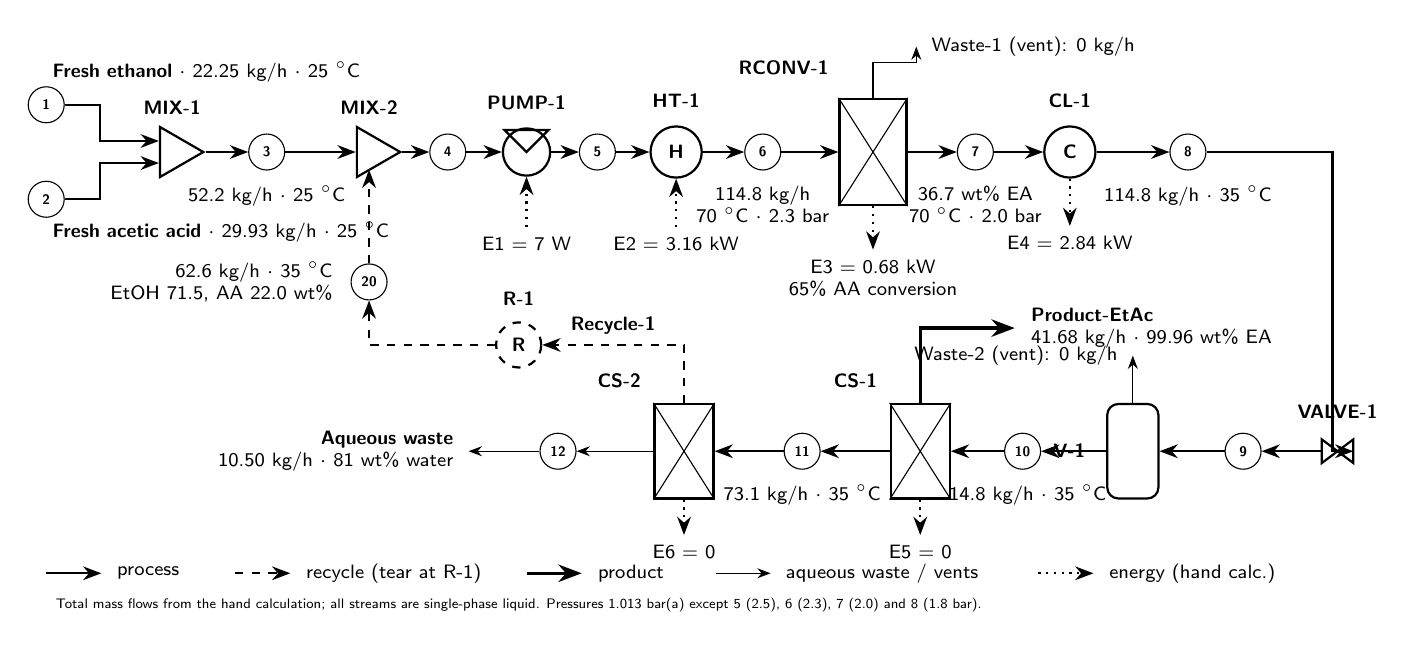
\begin{tikzpicture}[
    font=\sffamily\scriptsize,
    >=Stealth,
    stream/.style={->, thick, black},
    recstream/.style={->, thick, dashed, black},
    prodstream/.style={->, very thick, black},
    wastestream/.style={->, thin, black},
    enstream/.style={->, dotted, thick, black},
    stag/.style={circle, draw=black, fill=white, inner sep=1.2pt, minimum size=13pt, font=\sffamily\tiny\bfseries},
    unit/.style={draw=black, thick, fill=white, font=\sffamily\scriptsize\bfseries}
]

% --- TOP ROW: MIX-1 -> MIX-2 -> PUMP-1 -> HT-1 -> RCONV-1 -> CL-1 ---
% Feed 1 & 2
\node[stag] (s1) at (0, 3.6) {1};
\node[stag] (s2) at (0, 2.4) {2};
\node[above right=0pt and -6pt of s1, align=left] {\textbf{Fresh ethanol} $\cdot$ 22.25 kg/h $\cdot$ 25 $^\circ$C};
\node[below right=0pt and -6pt of s2, align=left] {\textbf{Fresh acetic acid} $\cdot$ 29.93 kg/h $\cdot$ 25 $^\circ$C};

% MIX-1 (triangle pointing right)
\node[unit, isosceles triangle, isosceles triangle apex angle=60, minimum height=0.55cm] (mix1) at (1.6, 3.0) {};
\node[above=3pt of mix1] {\textbf{MIX-1}};
\draw[stream] (s1.east) -- ++(0.45,0) |- ($(mix1.west)+(0,0.14)$);
\draw[stream] (s2.east) -- ++(0.45,0) |- ($(mix1.west)+(0,-0.14)$);

% Stream 3
\node[stag] (s3) at (2.8, 3.0) {3};
\node[below=2pt of s3, align=center] {52.2 kg/h $\cdot$ 25 $^\circ$C};
\draw[stream] (mix1.east) -- (s3.west);

% MIX-2
\node[unit, isosceles triangle, isosceles triangle apex angle=60, minimum height=0.55cm] (mix2) at (4.1, 3.0) {};
\node[above=3pt of mix2] {\textbf{MIX-2}};
\draw[stream] (s3.east) -- (mix2.west);

% Stream 4
\node[stag] (s4) at (5.1, 3.0) {4};
\draw[stream] (mix2.east) -- (s4.west);

% PUMP-1
\node[unit, circle, minimum size=0.6cm] (pump) at (6.1, 3.0) {};
\draw[thick] (pump.center) -- ++(0.28,0.28) -- ++(-0.56,0) -- cycle;
\node[above=3pt of pump] {\textbf{PUMP-1}};
\draw[stream] (s4.east) -- (pump.west);
\draw[enstream] (6.1, 2.05) -- (pump.south);
\node[below] at (6.1, 2.05) {E1 = 7 W};

% Stream 5
\node[stag] (s5) at (7.0, 3.0) {5};
\draw[stream] (pump.east) -- (s5.west);

% HT-1
\node[unit, circle, minimum size=0.65cm] (ht1) at (8.0, 3.0) {H};
\node[above=3pt of ht1] {\textbf{HT-1}};
\draw[stream] (s5.east) -- (ht1.west);
\draw[enstream] (8.0, 2.05) -- (ht1.south);
\node[below] at (8.0, 2.05) {E2 = 3.16 kW};

% Stream 6
\node[stag] (s6) at (9.1, 3.0) {6};
\node[below=2pt of s6, align=center] {114.8 kg/h\\70 $^\circ$C $\cdot$ 2.3 bar};
\draw[stream] (ht1.east) -- (s6.west);

% RCONV-1
\node[unit, rectangle, minimum width=0.85cm, minimum height=1.35cm] (rconv) at (10.5, 3.0) {};
\draw[thin] (rconv.north west) -- (rconv.south east) (rconv.south west) -- (rconv.north east);
\node[above=5pt of rconv.north west, anchor=south east] {\textbf{RCONV-1}};
\draw[stream] (s6.east) -- (rconv.west);
% Waste-1
\draw[wastestream] (rconv.north) -- ++(0,0.45) -- ++(0.55,0) -- ++(0,0.2) node[right=2pt] {Waste-1 (vent): 0 kg/h};
% E3
\draw[enstream] (rconv.south) -- ++(0,-0.55) node[below, align=center] {E3 = 0.68 kW\\65\% AA conversion};

% Stream 7
\node[stag] (s7) at (11.8, 3.0) {7};
\node[below=2pt of s7, align=center] {36.7 wt\% EA\\70 $^\circ$C $\cdot$ 2.0 bar};
\draw[stream] (rconv.east) -- (s7.west);

% CL-1
\node[unit, circle, minimum size=0.65cm] (cl1) at (13.0, 3.0) {C};
\node[above=3pt of cl1] {\textbf{CL-1}};
\draw[stream] (s7.east) -- (cl1.west);
\draw[enstream] (cl1.south) -- ++(0,-0.6) node[below] {E4 = 2.84 kW};

% Stream 8
\node[stag] (s8) at (14.5, 3.0) {8};
\node[below=2pt of s8] {114.8 kg/h $\cdot$ 35 $^\circ$C};
\draw[stream] (cl1.east) -- (s8.west);

% --- BOTTOM ROW (RIGHT TO LEFT): VALVE-1 -> V-1 -> CS-1 -> CS-2 -> R-1 ---
% VALVE-1
\node[draw=none, minimum size=0.4cm] (vpos) at (16.4, -0.8) {};
\draw[thick, fill=white] (16.2,-0.65) -- (16.2,-0.95) -- (16.6,-0.65) -- (16.6,-0.95) -- cycle;
\node[above=4pt] at (16.4,-0.65) {\textbf{VALVE-1}};
\draw[stream] (s8.east) -- ++(1.6,0) |- (16.6,-0.8);

% Stream 9
\node[stag] (s9) at (15.2, -0.8) {9};
\draw[stream] (16.2,-0.8) -- (s9.east);

% V-1
\node[unit, rectangle, rounded corners=4pt, minimum width=0.65cm, minimum height=1.2cm] (v1) at (13.8, -0.8) {};
\node[left=4pt of v1] {\textbf{V-1}};
\draw[stream] (s9.west) -- (v1.east);
\draw[wastestream] (v1.north) -- ++(0,0.6) node[left=2pt] {Waste-2 (vent): 0 kg/h};

% Stream 10
\node[stag] (s10) at (12.4, -0.8) {10};
\node[below=2pt of s10] {114.8 kg/h $\cdot$ 35 $^\circ$C};
\draw[stream] (v1.west) -- (s10.east);

% CS-1
\node[unit, rectangle, minimum width=0.75cm, minimum height=1.2cm] (cs1) at (11.1, -0.8) {};
\draw[thin] (cs1.north west) -- (cs1.south east) (cs1.south west) -- (cs1.north east);
\node[above left=2pt and 1pt of cs1] {\textbf{CS-1}};
\draw[stream] (s10.west) -- (cs1.east);
\draw[prodstream] (cs1.north) -- ++(0,0.95) -- ++(1.2,0) node[right=2pt, align=left] {\textbf{Product-EtAc}\\41.68 kg/h $\cdot$ 99.96 wt\% EA};
\draw[enstream] (cs1.south) -- ++(0,-0.45) node[below] {E5 = 0};

% Stream 11
\node[stag] (s11) at (9.6, -0.8) {11};
\node[below=2pt of s11] {73.1 kg/h $\cdot$ 35 $^\circ$C};
\draw[stream] (cs1.west) -- (s11.east);

% CS-2
\node[unit, rectangle, minimum width=0.75cm, minimum height=1.2cm] (cs2) at (8.1, -0.8) {};
\draw[thin] (cs2.north west) -- (cs2.south east) (cs2.south west) -- (cs2.north east);
\node[above left=2pt and 1pt of cs2] {\textbf{CS-2}};
\draw[stream] (s11.west) -- (cs2.east);
\draw[enstream] (cs2.south) -- ++(0,-0.45) node[below] {E6 = 0};

% Stream 12 (Aqueous waste)
\node[stag] (s12) at (6.5, -0.8) {12};
\draw[wastestream] (cs2.west) -- (s12.east);
\draw[wastestream] (s12.west) -- ++(-0.9,0) node[left=2pt, align=right] {\textbf{Aqueous waste}\\10.50 kg/h $\cdot$ 81 wt\% water};

% Recycle loop: CS-2 -> R-1 -> Stream 20 -> MIX-2
\node[unit, circle, dashed, minimum size=0.55cm] (r1) at (6.0, 0.55) {R};
\node[above=2pt of r1] {\textbf{R-1}};
\draw[recstream] (cs2.north) |- node[pos=0.75, above] {\textbf{Recycle-1}} (r1.east);

\node[stag] (s20) at (4.1, 1.35) {20};
\node[left=3pt of s20, align=right] {62.6 kg/h $\cdot$ 35 $^\circ$C\\EtOH 71.5, AA 22.0 wt\%};
\draw[recstream] (r1.west) -| (s20.south);
\draw[recstream] (s20.north) -- ($(mix2.south)+(0,0.02)$);

% Legend
\draw[stream] (0.0, -2.35) -- (0.7, -2.35) node[right=2pt] {process};
\draw[recstream] (2.4, -2.35) -- (3.1, -2.35) node[right=2pt] {recycle (tear at R-1)};
\draw[prodstream] (6.1, -2.35) -- (6.8, -2.35) node[right=2pt] {product};
\draw[wastestream] (8.5, -2.35) -- (9.2, -2.35) node[right=2pt] {aqueous waste / vents};
\draw[enstream] (12.6, -2.35) -- (13.3, -2.35) node[right=2pt] {energy (hand calc.)};

\node[anchor=west, font=\sffamily\tiny] at (0.0, -2.75) {Total mass flows from the hand calculation; all streams are single-phase liquid. Pressures 1.013 bar(a) except 5 (2.5), 6 (2.3), 7 (2.0) and 8 (1.8 bar).};

\end{tikzpicture}%
}
\caption{Process flow diagram with the hand-calculated flows, temperatures and duties. Equipment and stream tags are those of the DWSIM model (Appendix~A); the lower row runs from right to left.}
\label{fig:pfd}
\end{figure}

\subsection{Design Basis and Component Data}

Tables~\ref{tab:design_basis} and~\ref{tab:pure_comp} set out the plant design basis (production capacity, product purity specification, reactor operating conditions and equipment pressure-drop allowances) together with the pure-component physical and hazard properties (molar masses, boiling and melting points, flash points, flammability limits and UK workplace exposure limits) that govern phase behaviour and process safety.

\subsection{Separation Model and Conceptual Topology}

\textbf{Separation model.} The CS-1 and CS-2 splits are design targets (Appendix~A). CS-1 sends 99\% of the ester to the product with 0.01\% of the ethanol, 0.005\% of the acid and 0.08\% of the water, which meets the product specification. CS-2 recycles 99\% of the ethanol and of the remaining ester, 90\% of the acid and 30\% of the water. Recycling some water keeps the recycle at 92.5~wt\% ethanol on an ethanol--water basis, below the ethanol--water azeotrope (about 96~wt\%~\cite{ref7}), which a real column could not cross.

\textbf{Conceptual topology.} Cooling the 70~$^\circ$C effluent to 35~$^\circ$C in CL-1 and flashing it in V-1 is a simplification that suits the black-box separators: it keeps the let-down liquid 41~K below its bubble point (only 5.6~K without CL-1), so V-1 sees no vapour. In a rigorous plant the hot effluent would feed the first distillation column directly, after the feed--effluent exchanger of Section~\ref{sec:heat_int}, rather than being cooled only to be reboiled; CL-1 would shrink to a trim cooler, and V-1 would serve only as a surge and emergency knock-out drum, for example if the cooling water failed.

\begin{table}[H]
\centering
\caption{Design basis.}
\label{tab:design_basis}
\small
\begin{tabularx}{\textwidth}{|L{3.1cm}|Y|}
\hline
\hdrrow
\textbf{Parameter} & \textbf{Value and status} \\
\hline
Production & 1,000~kg/day of EA (41.67~kg/h), 24~h/day for 330~days/year (330~t/year) \\
\hline
Product & $\ge 99.8$~wt\% EA; water and ethanol $\le 300$~ppm; acidity $\le 50$~ppm as AA~\cite{ref3} \\
\hline
Feeds & Pure ethanol and pure acetic acid at 25~$^\circ$C and 1.01325~bar (assumed) \\
\hline
Reactor & 65\% single-pass AA conversion (assumed); 70~$^\circ$C, 2.3~bar inlet, isothermal; EtOH:AA = 2.00 at the inlet (design choice, Section~\ref{sec:eq_limit}) \\
\hline
Pressures & PUMP-1 2.5~bar; pressure drops HT-1 0.2~bar, RCONV-1 0.3~bar, CL-1 0.2~bar (allowances, Section~\ref{sec:kinetics}) \\
\hline
Separators & Fixed component splits (Section~2.3 and Appendix~A) \\
\hline
Property method & NRTL with ideal vapour (Section~\ref{sec:thermo}) \\
\hline
\end{tabularx}
\end{table}

\begin{table}[H]
\centering
\caption{Pure-component and hazard data.}
\label{tab:pure_comp}
\small
\begin{tabular}{|L{2.2cm}|R{1.6cm}|R{1.1cm}|R{1.1cm}|R{1.3cm}|R{1.5cm}|C{2.0cm}|C{2.2cm}|}
\hline
\hdrrow
\textbf{Compound} & \textbf{$M$ (kg/kmol)} & \textbf{$T_{\mathrm{b}}$ ($^\circ$C)} & \textbf{$T_{\mathrm{m}}$ ($^\circ$C)} & \textbf{Specific gravity} & \textbf{Flash point ($^\circ$C)} & \textbf{Flammable range (vol\%)} & \textbf{WEL 8~h / 15~min (ppm)} \\
\hline
Ethanol & 46.07 & 78 & $-114$ & 0.79 & 13 & 3.3--19 & 1,000 / -- \\
\hline
Acetic acid & 60.05 & 118 & 16.6 & 1.05 & 39 & 4.0--19.9 & 10 / 20 \\
\hline
Ethyl acetate & 88.11 & 77 & $-83$ & 0.90 & $-4$ & 2.0--11.5 & 200 / 400 \\
\hline
Water & 18.02 & 100 & 0 & 1.00 & -- & -- & -- \\
\hline
\end{tabular}
\tabnote{Molar masses as in DWSIM; other properties from the NIOSH pocket guide~\cite{ref4} (converted from $^\circ$F), the acetic acid melting point from NIST~\cite{ref5} and the UK workplace exposure limits (WEL) from EH40~\cite{ref6}.}
\end{table}

% ==================== SECTION 3 ====================
\section{Reaction Thermodynamics, Equilibrium and Reactor Sizing}

\subsection{Heat of Reaction}

The standard heat of reaction follows from the liquid formation enthalpies,
\begin{equation}
\Delta_{\mathrm{r}}H^\circ = \sum_i \nu_i \,\Delta_{\mathrm{f}}H_i^\circ(\mathrm{l}) = \Delta_{\mathrm{f}}H_{\mathrm{EA}}^\circ + \Delta_{\mathrm{f}}H_{\mathrm{W}}^\circ - \Delta_{\mathrm{f}}H_{\mathrm{AA}}^\circ - \Delta_{\mathrm{f}}H_{\mathrm{EtOH}}^\circ
\label{eq:hrxn}
\end{equation}
where $\nu_i$ is the stoichiometric coefficient. The most precise NIST values~\cite{ref5} give $\Delta_{\mathrm{r}}H^\circ = -5.27$~kJ/mol at 25~$^\circ$C and $-5.18$~kJ/mol at 70~$^\circ$C, with a range of $-6.9$ to $-2.5$~kJ/mol across other published formation enthalpies. The reaction is only mildly exothermic: at the design extent of reaction, 0.4730~kmol/h, the bed releases 0.68~kW, which would warm the liquid by only 8.0~K if no heat were removed. DWSIM's conversion reactor uses ideal-gas formation enthalpies instead, which give $-18.56$~kJ/mol~\cite{ref8}; the difference is the vaporisation enthalpies of the four components (Section~\ref{sec:duties}).

\subsection{Equilibrium Limit and Choice of Feed Ratio}
\label{sec:eq_limit}

On a mole-fraction basis the equilibrium constant is
\begin{equation}
K = \frac{x_{\mathrm{EA}}\,x_{\mathrm{W}}}{x_{\mathrm{AA}}\,x_{\mathrm{EtOH}}}
\label{eq:keq}
\end{equation}
where $x_i$ is the liquid mole fraction. Because DWSIM's conversion reactor imposes whatever single-pass conversion is entered without checking chemical equilibrium, the assumed 65\% target must be verified independently against the equilibrium ceiling $X_{\mathrm{eq}}$. Published values of $K$ are 2.77 at 70~$^\circ$C from the kinetic fit of Lai et~al.~\cite{ref7}, 3.98 at 80~$^\circ$C~\cite{ref9} and the classic 4.0 for an equimolar mixture~\cite{ref10}. For an equimolar feed, $X_{\mathrm{eq}} = \sqrt{K}/(1+\sqrt{K})$, which gives only 62--67\%, so 65\% would sit at or beyond equilibrium. The design therefore feeds ethanol in excess. At $\mathrm{EtOH:AA} = 2.0$, with the recycled water and ester included, the equilibrium ceiling rises to 76.5--81.2\% (Table~\ref{tab:eq_cat}); Figure~\ref{fig:tradeoffs} shows the trade-off with the recycle flow.

Equation~\eqref{eq:keq} treats the liquid as ideal. Accounting for non-ideal molecular interactions in this polar liquid requires thermodynamic activities, $a_i = \gamma_i x_i$~\cite{ref11}:
\begin{equation}
K_a = K_x\,\Gamma, \qquad \Gamma = \frac{\gamma_{\mathrm{EA}}\,\gamma_{\mathrm{W}}}{\gamma_{\mathrm{AA}}\,\gamma_{\mathrm{EtOH}}}
\label{eq:ka}
\end{equation}
where $K_x$ is the mole-fraction ratio of Equation~\eqref{eq:keq} and $\gamma_i$ the NRTL activity coefficient. Calibrating on the classic equimolar equilibrium ($K_x = 4.0$, where NRTL gives $\Gamma = 3.82$ at 25~$^\circ$C) gives $K_a = 15.3$; the van~'t~Hoff equation with $\Delta_{\mathrm{r}}H^\circ$ lowers it to 11.6 at 70~$^\circ$C. Because $\Gamma$ is larger in the ethanol-rich reactor liquid (5.2), the activity basis lowers the estimated equilibrium conversion to 73.5--77.3\%. Because this screening estimate is calibrated from an approximate historical equimolar constant rather than experimental measurements on this exact quaternary feed mixture, the 73.5--81.2\% range represents model-dependent estimates rather than experimentally established limits; even at the lowest estimate, 65\% is 88\% of equilibrium and the catalyst needed rises only from 15.4 to 16.5~kg.

\begin{table}[H]
\centering
\caption{Equilibrium conversion at the reactor inlet ($\mathrm{EtOH:AA} = 2.0$) and catalyst for 65\% conversion.}
\label{tab:eq_cat}
\small
\begin{tabularx}{\textwidth}{|Y|C{1.1cm}|R{1.6cm}|R{1.2cm}|R{1.6cm}|R{1.4cm}|R{1.4cm}|}
\hline
\hdrrow
\textbf{Basis} & \textbf{$T$ ($^\circ$C)} & \textbf{$K$} & \textbf{$X_{\mathrm{eq}}$} & \textbf{65\% as share of $X_{\mathrm{eq}}$} & \textbf{Plug flow (kg)} & \textbf{Stirred tank (kg)} \\
\hline
Lai et~al.\ kinetic fit~\cite{ref7} & 60 & 2.67 & 76.0\% & 86\% & 25.8 & 84.0 \\
\hline
Lai et~al.\ kinetic fit~\cite{ref7} (design) & 70 & 2.77 & 76.5\% & 85\% & 15.4 & 48.9 \\
\hline
Lai et~al.\ kinetic fit~\cite{ref7} & 80 & 2.87 & 77.0\% & 84\% & 9.5 & 29.5 \\
\hline
\.{I}nce~\cite{ref9} & 80 & 3.98 & 81.2\% & 80\% & -- & -- \\
\hline
Classic equimolar value~\cite{ref10} & room & 4.0 & 81.2\% & 80\% & -- & -- \\
\hline
NRTL activity basis, $K_a$ independent of $T$ & 70 & 15.3 ($K_a$) & 77.3\% & 84\% & -- & -- \\
\hline
NRTL activity basis, van~'t~Hoff & 70 & 11.6 ($K_a$) & 73.5\% & 88\% & 16.5 & -- \\
\hline
\end{tabularx}
\tabnote{Catalyst is wet Amberlyst~35. The last row's catalyst mass uses the kinetic model with its equilibrium moved to that limit.}
\end{table}

\textbf{Note on the temperature trend.} Table~\ref{tab:eq_cat} contains an apparent contradiction. Lai's $K = k_1/k_{-1}$ rises from 2.67 at 60~$^\circ$C to 2.87 at 80~$^\circ$C because $E_{a,1}/R = 6105.6$~K exceeds $E_{a,-1}/R = 5692.1$~K, which implies an apparent, endothermic reaction enthalpy of $+3.4$~kJ/mol; the calorimetric value of Section~3.1 is $-5.3$~kJ/mol, so the true constant should fall. When $|\Delta_{\mathrm{r}}H|$ is this small, a fit in concentrations absorbs the temperature dependence of the activity coefficients into its apparent activation energies: with NRTL, $\Gamma$ falls as the temperature rises, so $K_x = K_a/\Gamma$ falls only half as fast as $K_a$ (apparent enthalpy $-2.5$~kJ/mol). The rest reflects how weak, and hard to fit, the dependence is: between 60 and 80~$^\circ$C either trend changes $K$ by less than 8\%. The activity-based check therefore governs the equilibrium limit and its temperature trend, and Lai's model is used only locally, at 70~$^\circ$C, to size the bed.

\subsection{Kinetics and Reactor Sizing}
\label{sec:kinetics}

The bed is sized with the pseudo-homogeneous rate law of Lai et~al.\ for Amberlyst~35~\cite{ref7}:
\begin{equation}
r' = k_1 C_{\mathrm{AA}} C_{\mathrm{EtOH}} - k_{-1} C_{\mathrm{EA}} C_{\mathrm{W}}, \qquad
k_1 = 1.24 \times 10^9\, e^{-6105.6/T}, \qquad
k_{-1} = 1.34 \times 10^8\, e^{-5692.1/T}
\label{eq:rate}
\end{equation}
where $r'$ is the rate per gram of wet catalyst ($\mathrm{mol\,g^{-1}\,min^{-1}}$), $C_i$ the concentration ($\mathrm{mol/cm^3}$), $k_1$ and $k_{-1}$ the forward and reverse rate constants ($\mathrm{cm^6\,mol^{-1}\,g^{-1}\,min^{-1}}$) and $T$ the temperature (K). For an isothermal plug-flow bed and a stirred tank,
\begin{equation}
W_{\mathrm{PFR}} = F_{\mathrm{AA},0} \int_0^X \frac{\mathrm{d}X'}{r'(X')}, \qquad
W_{\mathrm{CSTR}} = \frac{F_{\mathrm{AA},0}\, X}{r'(X)}
\label{eq:sizing}
\end{equation}
where $F_{\mathrm{AA},0}$ is the acetic acid molar flow at the reactor inlet (mol/min), so $W$ comes out in grams and is converted to kilograms. A well-mixed stirred tank (CSTR) needs about three times the catalyst mass of a plug-flow bed (PFR, Table~\ref{tab:eq_cat}) because it operates everywhere at the low outlet reactant concentrations, where the reverse reaction nearly cancels the forward rate; a fixed plug-flow bed is therefore chosen. The design catalyst inventory is set by the larger of 1.25 times the kinetic mass (25\% ageing margin) and the mass needed to keep the liquid hourly space velocity (LHSV, defined as volumetric liquid feed rate divided by bed volume) within the catalyst data-sheet maximum of 5~BV/h~\cite{ref12}. Here the space-velocity limit governs, giving a bed 0.20~m in diameter and 1.0~m deep holding 25.1~kg of wet resin (LHSV 4.4~h$^{-1}$). The Ergun equation predicts a clean-bed pressure drop ($\Delta P$) of only 1.1~kPa (0.011~bar). The 0.3~bar allowance used in DWSIM is a deliberate, conservative design margin for the distributor, support screen, resin swelling and fouling; a smaller pressure drop would only raise downstream pressures and widen the boiling margins of Section~\ref{sec:phase}.

% ==================== SECTION 4 ====================
\section{Thermodynamic Model Selection and NRTL Validation}
\label{sec:thermo}

\subsection{Choice of NRTL}

All four components are polar and three of them hydrogen-bond, so the liquid deviates strongly from Raoult's law: the system has three binary azeotropes and a ternary one, and ethyl acetate is only partly miscible with water. A cubic equation of state such as Peng--Robinson cannot represent this with its standard parameters, so an activity-coefficient model is needed. NRTL represents both vapour--liquid and liquid--liquid equilibrium with binary parameters, $\tau_{ij} = A_{ij}/RT$ and $G_{ij} = \exp(-\alpha_{ij}\tau_{ij})$. With an ideal vapour, DWSIM's default, bubble points follow from the modified Raoult's law,
\begin{equation}
P = \sum_i x_i\,\gamma_i\, P_i^{\mathrm{sat}}(T)
\label{eq:raoult}
\end{equation}
where $P_i^{\mathrm{sat}}$ is the vapour pressure. DWSIM's database holds only four of the six pairs; it estimates the two acetic-acid pairs from the UNIFAC group-contribution method (Table~\ref{tab:nrtl}). The estimate is uncertain, but replacing it changes the bubble temperatures of the process streams by less than 0.5~K.

\begin{table}[H]
\centering
\caption{NRTL parameters used by DWSIM.}
\label{tab:nrtl}
\small
\begin{tabularx}{\textwidth}{|L{4.0cm}|R{2.1cm}|R{2.1cm}|R{1.1cm}|Y|}
\hline
\hdrrow
\textbf{Pair $i$ / $j$} & \textbf{$A_{ij}$ (cal/mol)} & \textbf{$A_{ji}$ (cal/mol)} & \textbf{$\alpha_{ij}$} & \textbf{Source} \\
\hline
Ethanol / acetic acid & $-34.20$ & $-190.78$ & 0.305 & DWSIM database (DECHEMA) \\
\hline
Ethanol / water & $-57.96$ & 1,241.74 & 0.294 & DWSIM database \\
\hline
Ethyl acetate / ethanol & 305.60 & 330.51 & 0.299 & DWSIM database (DECHEMA) \\
\hline
Ethyl acetate / water & 1,285.99 & 1,606.08 & 0.439 & DWSIM database (DECHEMA) \\
\hline
Acetic acid / water & $-189.1$ & 728.8 & 0.200 & Estimated by DWSIM from UNIFAC \\
\hline
Acetic acid / ethyl acetate & $-303.6$ & 544.8 & 0.200 & Estimated by DWSIM from UNIFAC \\
\hline
\end{tabularx}
\tabnote{$R = 1.98721\text{ cal/(mol K)}$ in $\tau_{ij}$. Values as stored in both solved DWSIM files.}
\end{table}

\begin{table}[H]
\centering
\caption{Azeotropes at 1.013~bar: literature against NRTL with the DWSIM parameters.}
\label{tab:azeotropes}
\small
\begin{tabularx}{\textwidth}{|C{3.1cm}|Z|Z|C{1.8cm}|}
\hline
\hdrrow
\textbf{Azeotrope} & \textbf{Literature~\cite{ref7}} & \textbf{NRTL (DWSIM set)} & \textbf{Difference} \\
\hline
Ethyl acetate--ethanol & 71.81~$^\circ$C, $x_{\mathrm{EA}} = 0.538$ & 72.04~$^\circ$C, $x_{\mathrm{EA}} = 0.552$ & $+0.23$~K \\
\hline
Ethanol--water & 78.17~$^\circ$C, $x_{\mathrm{EtOH}} = 0.904$ & 78.38~$^\circ$C, $x_{\mathrm{EtOH}} = 0.868$ & $+0.21$~K \\
\hline
Ethyl acetate--water & 70.38~$^\circ$C, $x_{\mathrm{EA}} = 0.689$ & 70.50~$^\circ$C, $x_{\mathrm{EA}} = 0.714$ & $+0.12$~K \\
\hline
EA--EtOH--water & 70.23~$^\circ$C; EA 0.579, EtOH 0.113 & 70.47~$^\circ$C; EA 0.666, EtOH 0.073 & $+0.24$~K \\
\hline
Acetic acid--water & None & 99.83~$^\circ$C, $x_{\mathrm{AA}} = 0.077$ & Spurious \\
\hline
\end{tabularx}
\tabnote{Compositions are mole fractions.}
\end{table}

\subsection{Validation Against Literature Data}

Table~\ref{tab:azeotropes} shows that the azeotrope temperatures are reproduced within 0.3~K and the binary compositions within 0.04~mole fraction, which is adequate for the single-phase subcooling checks. However, three limitations matter for separation design. First, the predicted ternary ethyl acetate--ethanol--water azeotrope composition differs by 0.087~mole fraction in ethyl acetate (0.666 vs.\ 0.579), a substantial compositional error despite the small temperature difference (+0.24~K). Second, the estimated acetic acid--water pair, paired with an ideal vapour that ignores acetic acid dimerisation, predicts a spurious azeotrope that does not exist; it does not affect this flowsheet, but an acid-recovery column designed with it would be wrong. Third, the ethyl acetate--water pair was fitted to vapour--liquid data: at 25~$^\circ$C it predicts an aqueous layer with $x_{\mathrm{EA}} = 0.077$, about four times the measured solubility ($x_{\mathrm{EA}} \approx 0.018$~\cite{ref13}), so the miscibility gap is far too narrow. A decanter and rigorous distillation train must therefore use liquid--liquid parameters, such as those of Trofimova et~al.~\cite{ref14}.

\subsection{Phase Stability and Subcooling Checks}
\label{sec:phase}

Every process stream was checked for boiling (vapour formation) and for splitting into two immiscible liquid layers. To check for boiling, the bubble point of each stream at its operating pressure is compared with its temperature: the reactor feed at 2.3~bar boils at 110.0~$^\circ$C (40~K above the 70~$^\circ$C reactor temperature), the effluent at 2.0~bar has a 25~K subcooling margin, and after CL-1 and the let-down valve the liquid is 41~K subcooled. To check for liquid--liquid phase splitting, the Python script performs a Gibbs tangent-plane stability test (checking whether splitting into an organic ester-rich layer and an aqueous layer lowers total Gibbs free energy); no split is found anywhere in the flowsheet because the high ethanol concentration acts as a mutual co-solvent that keeps ester and water in a single liquid phase. Both solved DWSIM runs agree, with zero flow in both vents. Because DWSIM's default flash only checks vapour--liquid equilibrium (VLE), any future decanter model must explicitly switch the flash algorithm to vapour--liquid--liquid equilibrium (VLLE).

% ==================== SECTION 5 ====================
\section{Mass Balance, Recycle Snowball Effect and Solver Validation}

\subsection{Stream Results}

The steady state is solved in closed form. The fraction of each component that goes round the loop again is its loop gain,
\begin{equation}
g_i = (1 - s_i)\, r_i
\label{eq:gain}
\end{equation}
where $s_i$ is the fraction sent to the product by CS-1 and $r_i$ the fraction recycled by CS-2. With the acetic acid flow at the reactor inlet fixed by the production rate and the ethanol flow by the 2:1 ratio, each fresh feed only has to replace what reacts and what is lost. The fresh EtOH:AA ratio is therefore 0.97, below stoichiometric, because more acid than ethanol leaves in the waste. Table~\ref{tab:streams} gives the stream results. In both DWSIM runs the external mass balance closes within $3.5 \times 10^{-5}$~kg/h, or 0.00007\% of the fresh feed, and the hand calculation's unit, overall and carbon, hydrogen and oxygen balances close to machine precision.

\begin{table}[H]
\centering
\caption{Process stream table (hand calculation) with the largest difference of the two solved DWSIM runs.}
\label{tab:streams}
\scriptsize
\setlength{\tabcolsep}{3.5pt}
\begin{tabular}{|L{1.65cm}|L{2.25cm}|R{0.8cm}|R{0.8cm}|R{1.0cm}|R{1.05cm}|R{1.0cm}|R{1.0cm}|R{0.9cm}|R{0.95cm}|R{1.25cm}|}
\hline
\hdrrow
\textbf{Stream} & \textbf{Description} & \textbf{$T$ ($^\circ$C)} & \textbf{$P$ (bar)} & \textbf{Mass (kg/h)} & \textbf{Molar (kmol/h)} & \textbf{EtOH (wt\%)} & \textbf{AA (wt\%)} & \textbf{EA (wt\%)} & \textbf{Water (wt\%)} & \textbf{DWSIM $-$ hand (\%)} \\
\hline
1 & Fresh Ethanol & 25.0 & 1.01 & 22.25 & 0.483 & 100.00 & 0 & 0 & 0 & $+0.0001$ \\
\hline
2 & Fresh Acetic Acid & 25.0 & 1.01 & 29.93 & 0.498 & 0 & 100.00 & 0 & 0 & $-0.0001$ \\
\hline
3 & MIX-1 outlet & 25.0 & 1.01 & 52.18 & 0.981 & 42.63 & 57.37 & 0 & 0 & $0.0000$ \\
\hline
20 & Recycle to MIX-2 & 35.0 & 1.01 & 62.62 & 1.409 & 71.53 & 21.98 & 0.67 & 5.82 & $-0.0062$ \\
\hline
4 & MIX-2 outlet & 30.7 & 1.01 & 114.80 & 2.390 & 58.40 & 38.06 & 0.36 & 3.18 & $-0.0034$ \\
\hline
5 & PUMP-1 outlet & 30.8 & 2.50 & 114.80 & 2.390 & 58.40 & 38.06 & 0.36 & 3.18 & $-0.0034$ \\
\hline
6 & Reactor feed & 70.0 & 2.30 & 114.80 & 2.390 & 58.40 & 38.06 & 0.36 & 3.18 & $-0.0034$ \\
\hline
Waste-1 & Reactor vent & -- & 2.00 & 0 & 0 & -- & -- & -- & -- & -- \\
\hline
7 & Reactor effluent & 70.0 & 2.00 & 114.80 & 2.390 & 39.42 & 13.32 & 36.66 & 10.60 & $-0.0034$ \\
\hline
8 & CL-1 outlet & 35.0 & 1.80 & 114.80 & 2.390 & 39.42 & 13.32 & 36.66 & 10.60 & $-0.0034$ \\
\hline
9 & Valve outlet & 35.0 & 1.01 & 114.80 & 2.390 & 39.42 & 13.32 & 36.66 & 10.60 & $-0.0034$ \\
\hline
Waste-2 & V-1 vent & -- & 1.01 & 0 & 0 & -- & -- & -- & -- & -- \\
\hline
10 & V-1 liquid & 35.0 & 1.01 & 114.80 & 2.390 & 39.42 & 13.32 & 36.66 & 10.60 & $-0.0034$ \\
\hline
Product-EtAc & Product & 35.0 & 1.01 & 41.68 & 0.474 & 0.01 & $<$0.01 & 99.96 & 0.02 & $0.0000$ \\
\hline
11 & CS-1 residue & 35.0 & 1.01 & 73.12 & 1.917 & 61.88 & 20.91 & 0.58 & 16.63 & $-0.0054$ \\
\hline
Recycle-1 & CS-2 recycle & 35.0 & 1.01 & 62.62 & 1.409 & 71.53 & 21.98 & 0.67 & 5.82 & $-0.0062$ \\
\hline
12 & Aqueous waste & 35.0 & 1.01 & 10.50 & 0.508 & 4.31 & 14.57 & 0.04 & 81.08 & $-0.0005$ \\
\hline
\end{tabular}
\tabnote{All streams are single-phase liquid. Last column: difference in total mass flow, the larger of the two runs; the largest difference in any component is 0.009\%. Temperatures assume ideal mixing (Section~\ref{sec:duties}).}
\end{table}

\textbf{Product quality.} Table~\ref{tab:spec} compares the product with the sales specification; the composition limits are met by construction of the CS-1 splits, and the specific gravity and boiling range are predicted with the property models.

\begin{table}[H]
\centering
\caption{Product (\texttt{Product-EtAc}) against the sales specification~\cite{ref3}.}
\label{tab:spec}
\small
\begin{tabularx}{\textwidth}{|Y|C{3.0cm}|R{2.4cm}|R{2.4cm}|}
\hline
\hdrrow
\textbf{Property} & \textbf{Test method} & \textbf{Limit} & \textbf{Predicted} \\
\hline
Ethyl acetate purity (wt\%) & ASTM D3545 & $\ge 99.8$ & 99.964 \\
\hline
Water (ppm) & ASTM E1064 & $\le 300$ & 234 \\
\hline
Ethanol (ppm) & ASTM D3545 & $\le 300$ & 109 \\
\hline
Acidity as acetic acid (ppm) & ASTM D1613 & $\le 50$ & 18 \\
\hline
Specific gravity at 20/20~$^\circ$C & ASTM D4052 & 0.900--0.903 & 0.9017 \\
\hline
Distillation range ($^\circ$C) & ASTM D1078 & 75.5--78.0 & 77.0--77.2 \\
\hline
\end{tabularx}
\tabnote{Colour (ASTM D1209), non-volatile matter (ASTM D1353) and residual odour (ASTM D1296) depend on trace impurities that the model does not represent and require laboratory testing.}
\end{table}

\subsection{Snowball Effect and Recycle Convergence}

It is important to distinguish physical ethanol circulation from perturbation sensitivity around the recycle loop. Physically, 32.5\% of reactor-inlet ethanol is consumed by reaction on each pass, and 99\% of the remaining unreacted ethanol is recycled by CS-2, so the surviving-and-recycled fraction per pass is $(1 - 0.325)(0.9999)(0.99) \approx 0.668$---corresponding to an average of only about 3.0 physical passages through the reactor per mole of fresh ethanol entering the plant ($1.455 / 0.483 = 3.01$). For flow perturbations, however, acetic acid is the limiting reactant that fixes the extent of reaction; any excess perturbation in fresh ethanol therefore passes through the reactor unreacted and circulates with a numerical loop gain of $g_{\mathrm{EtOH}} = (1 - s_{\mathrm{EtOH}})r_{\mathrm{EtOH}} = 0.990$ (amplification factor $1/(1-g) \approx 99$). Consequently, a 1\% error in stream~1 shifts the reactor-inlet ethanol flow by about a third. This is the snowball sensitivity described by Luyben~\cite{ref15}; in a real plant, fresh ethanol make-up would be set by inventory or ratio control rather than a fixed flow.

That same 0.990 numerical loop gain makes sequential flowsheet iteration slow to converge. In DWSIM, recycle block R-1 breaks the loop at a ``tear stream'' (stream~20), guesses its flow rate and composition, and updates them iteratively using direct substitution until successive passes differ by less than the specified mass-flow tolerance. DWSIM's default tolerance is 0.01~kg/s~\cite{ref8}---more than half of this plant's entire recycle flow (0.0174~kg/s). A Python reconstruction of DWSIM's default direct-substitution procedure, starting from an empty tear stream, predicts false convergence after just two iterations with the recycle stuck at 25.4~kg/h (41\% of its true value) and a reactor-inlet EtOH:AA ratio of 0.99 instead of 2.00 (Figure~\ref{fig:recycle}). At that ratio the model-estimated equilibrium ceiling is only 58\%, yet the conversion reactor still imposes 65\% because it does not check equilibrium. A ``converged'' run is therefore not proof of a physically valid solution. Both solved DWSIM files tighten the tolerance to $1 \times 10^{-8}$~kg/s (1,000-iteration limit, no acceleration), landing within 0.006\% of the exact steady state---matching the analytical truncation bound where a final step $\delta$ leaves an unconverged tail of $\delta\,g/(1-g) \approx 98\,\delta$.

\begin{figure}[H]
\centering
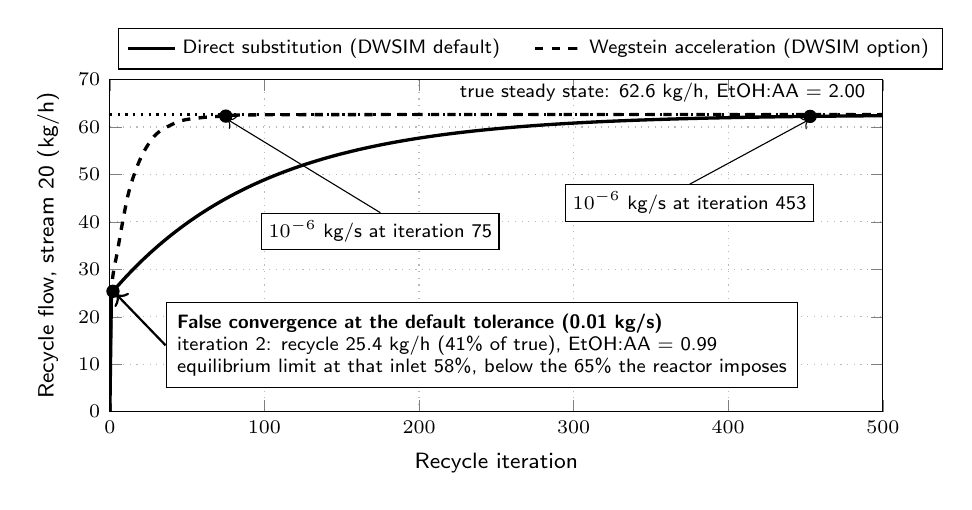
\begin{tikzpicture}
\begin{axis}[
    width=0.94\textwidth,
    height=5.8cm,
    xlabel={Recycle iteration},
    ylabel={Recycle flow, stream 20 (kg/h)},
    xmin=0, xmax=500,
    ymin=0, ymax=70,
    xtick={0,100,200,300,400,500},
    ytick={0,10,20,30,40,50,60,70},
    grid=both,
    grid style={dotted, gray!55},
    axis lines=box,
    tick label style={font=\sffamily\scriptsize},
    label style={font=\sffamily\footnotesize},
    legend style={at={(0.01,1.03)}, anchor=south west, legend columns=2, draw=black, font=\sffamily\scriptsize, /tikz/every even column/.append style={column sep=10pt}}
]
% True steady state line
\addplot[dotted, thick, black, domain=0:500, forget plot] {62.62};
\node[anchor=south east, font=\sffamily\scriptsize] at (axis cs:495,63.2) {true steady state: 62.6~kg/h, EtOH:AA = 2.00};

% Direct substitution curve
\addplot[solid, very thick, black, domain=1:500, samples=120] {62.62 - 37.62*(0.9899^(x-1))};
\addlegendentry{Direct substitution (DWSIM default)}

% Wegstein acceleration curve
\addplot[dashed, very thick, black, smooth] coordinates {
    (0,0) (1,25.0) (5,34.0) (12,46.0) (20,53.5) (30,58.5) (45,61.2) (60,62.0) (75,62.3) (120,62.6) (500,62.62)
};
\addlegendentry{Wegstein acceleration (DWSIM option)}

% Initial segment (0,0) to (1,25)
\addplot[solid, very thick, black, forget plot] coordinates {(0,0) (1,25.0)};

% Key points
\addplot[only marks, mark=*, mark size=2.2pt, black, forget plot] coordinates {(2,25.38) (75,62.3) (453,62.24)};

% Annotations
\node[draw=black, fill=white, align=left, font=\sffamily\scriptsize, inner sep=4pt, anchor=west] (fcbox) at (axis cs:36,14) {
    \textbf{False convergence at the default tolerance (0.01 kg/s)}\\
    iteration 2: recycle 25.4 kg/h (41\% of true), EtOH:AA = 0.99\\
    equilibrium limit at that inlet 58\%, below the 65\% the reactor imposes
};
\draw[->, thick, black] (fcbox.west) -- (axis cs:4,24.8);

\node[draw=black, fill=white, font=\sffamily\scriptsize, inner sep=2.5pt] (w75) at (axis cs:175,38) {$10^{-6}$~kg/s at iteration 75};
\draw[->, black] (w75.north) -- (axis cs:76,61.6);

\node[draw=black, fill=white, font=\sffamily\scriptsize, inner sep=2.5pt] (d453) at (axis cs:375,44) {$10^{-6}$~kg/s at iteration 453};
\draw[->, black] (d453.north) -- (axis cs:452,61.5);

\end{axis}
\end{tikzpicture}
\caption{Recycle flow against iteration on the DWSIM loop, from an empty tear stream (DWSIM's algorithm repeated in the script). Direct substitution needs 906 iterations to reach the $1 \times 10^{-8}$~kg/s used in the solved files.}
\label{fig:recycle}
\end{figure}

% ==================== SECTION 6 ====================
\section{DWSIM Validation, Enthalpy Sensitivity and Heat Integration}

\subsection{The Two Solved Runs}

Two DWSIM files were solved with identical inputs (Appendix~A) and differ only in the enthalpy method of the NRTL property package: Case~A uses DWSIM's default, Lee--Kesler, and Case~B uses ``Liquid Cp + Enthalpy of Vaporization''. The script reads each solved file directly, so no result is retyped. It compares every stream, duty and temperature with the hand calculation and with its own evaluation of the enthalpy method used, checks DWSIM's activity coefficients against its own NRTL routine (agreement within $8 \times 10^{-9}$) and checks the overall balances and the recycle convergence. The material results of the two runs are identical (largest stream difference $1 \times 10^{-4}$~kg/h), and all twelve acceptance checks pass in both (Table~\ref{tab:checks}).

\begin{table}[H]
\centering
\caption{Acceptance checks on the two solved DWSIM runs (all pass).}
\label{tab:checks}
\small
\begin{tabularx}{\textwidth}{|C{3.2cm}|Y|C{3.5cm}|C{3.5cm}|}
\hline
\hdrrow
\textbf{Check} & \textbf{Criterion} & \textbf{Case A (Lee--Kesler)} & \textbf{Case B (Liquid $C_p$)} \\
\hline
Product flow & Within 0.1\% of hand & 41.682~kg/h ($+0.00001\%$) & 41.682~kg/h ($+0.00001\%$) \\
\hline
Product purity & Within 0.01~wt\% & 99.964~wt\% & 99.964~wt\% \\
\hline
Reactor-inlet EtOH:AA & $2.000 \pm 0.005$ & 1.99988 & 1.99989 \\
\hline
Recycle, stream~20 & Within 0.1\% & 62.621~kg/h ($-0.0062\%$) & 62.621~kg/h ($-0.0060\%$) \\
\hline
Aqueous waste, stream~12 & Within 0.1\% & 10.497~kg/h ($-0.0005\%$) & 10.497~kg/h ($-0.0005\%$) \\
\hline
Vents Waste-1, Waste-2 & Zero & 0~kg/h & 0~kg/h \\
\hline
Phases & Single liquid everywhere & 15 streams liquid & 15 streams liquid \\
\hline
Duties E2--E6 & Within 1\% of the script's evaluation & within 0.02\% & within 0.01\% \\
\hline
Mixer temperatures $T_3$, $T_4$ & Within 0.1~K of the same & within 0.011~K & within 0.001~K \\
\hline
Overall mass balance & Residual below recycle tolerance & $9.6 \times 10^{-9}$~kg/s & $9.3 \times 10^{-9}$~kg/s \\
\hline
Overall energy balance & Closes within 0.01~kW & 0.0005~kW & 0.0001~kW \\
\hline
Final solve & No errors or warnings; converged & Clean; converged & Clean; converged \\
\hline
\end{tabularx}
\end{table}

\subsection{Duties: Two Enthalpy Methods against the Hand Calculation}
\label{sec:duties}

The hand calculation takes liquid enthalpies from the DIPPR heat capacities that DWSIM loads, which agree with NIST data within 2.2\%~\cite{ref5}, and the liquid-phase heat of reaction of Section~3.1; the pump work goes into the liquid. Table~\ref{tab:duties} and Figure~\ref{fig:duties} compare it with the two runs.

\begin{table}[H]
\centering
\caption{Duties (kW unless stated) and mixer temperatures: hand calculation and the two solved DWSIM runs.}
\label{tab:duties}
\small
\begin{tabularx}{\textwidth}{|Y|R{2.1cm}|R{2.1cm}|R{2.1cm}|R{1.9cm}|}
\hline
\hdrrow
\textbf{Quantity} & \textbf{Hand calculation} & \textbf{Case A Lee--Kesler} & \textbf{Case B Liquid $C_p$} & \textbf{Case B vs A} \\
\hline
E1, PUMP-1 shaft power (W) & 7.27 & 7.35 & 7.33 & $-0.3\%$ \\
\hline
E2, HT-1 heating & 3.161 & 3.675 & 3.165 & $-13.9\%$ \\
\hline
E3, RCONV-1 heat removal & 0.680 & 0.750 & 2.428 & $+223.6\%$ \\
\hline
E4, CL-1 heat removal & 2.842 & 3.387 & 2.842 & $-16.1\%$ \\
\hline
E5, CS-1 enthalpy imbalance & 0.000 & 0.285 & 0.000 & $-100.0\%$ \\
\hline
E6, CS-2 enthalpy imbalance & 0.000 & 0.186 & 0.000 & $-100.0\%$ \\
\hline
$T_3$, MIX-1 outlet ($^\circ$C) & 25.00 & 29.92 & 25.00 & $-4.92$~K \\
\hline
$T_4$, MIX-2 outlet ($^\circ$C) & 30.74 & 33.31 & 30.76 & $-2.55$~K \\
\hline
\end{tabularx}
\end{table}

\begin{figure}[H]
\centering
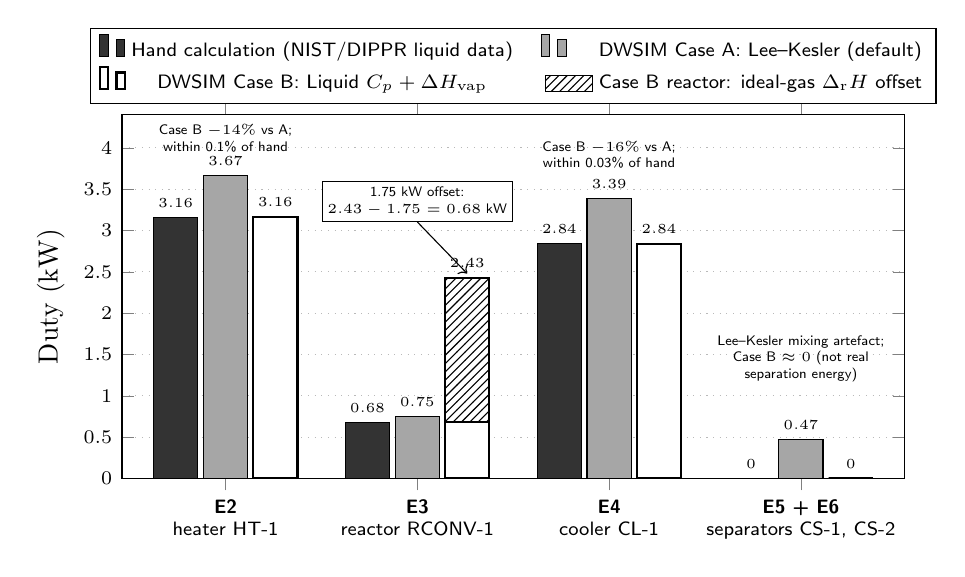
\begin{tikzpicture}
\begin{axis}[
    ybar=2pt,
    bar width=16pt,
    width=0.95\textwidth,
    height=6.2cm,
    ylabel={Duty (kW)},
    ymin=0, ymax=4.4,
    ytick={0,0.5,1.0,1.5,2.0,2.5,3.0,3.5,4.0},
    symbolic x coords={E2, E3, E4, E56},
    xtick=data,
    xticklabels={
        {\textbf{E2}\\heater HT-1},
        {\textbf{E3}\\reactor RCONV-1},
        {\textbf{E4}\\cooler CL-1},
        {\textbf{E5 + E6}\\separators CS-1, CS-2}
    },
    xticklabel style={align=center, font=\sffamily\scriptsize},
    yticklabel style={font=\sffamily\scriptsize},
    ylabel style={font=\sffamily\footnotesize},
    ymajorgrids=true,
    grid style={dotted, gray!55},
    axis lines=box,
    enlarge x limits=0.18,
    legend style={at={(0.5,1.03)}, anchor=south, legend columns=2, draw=black, font=\sffamily\scriptsize, /tikz/every even column/.append style={column sep=8pt}},
    nodes near coords,
    every node near coord/.append style={font=\sffamily\tiny, black, /pgf/number format/fixed, /pgf/number format/precision=2}
]

% 1. Hand calculation (dark charcoal)
\addplot[fill=barhand, draw=black] coordinates {(E2,3.16) (E3,0.68) (E4,2.84) (E56,0.00)};
\addlegendentry{Hand calculation (NIST/DIPPR liquid data)}

% 2. Case A Lee-Kesler (medium grey)
\addplot[fill=barlk, draw=black] coordinates {(E2,3.67) (E3,0.75) (E4,3.39) (E56,0.47)};
\addlegendentry{DWSIM Case A: Lee--Kesler (default)}

% 3. Case B Liquid Cp (white with thick black border; E3 bar plotted to 2.43 total, with hatched overlay drawn below)
\addplot[fill=white, draw=black, thick] coordinates {(E2,3.16) (E3,2.43) (E4,2.84) (E56,0.00)};
\addlegendentry{DWSIM Case B: Liquid $C_p + \Delta H_{\mathrm{vap}}$}

% Dummy legend entry for hatched offset
\addlegendimage{area legend, fill=white, pattern=north east lines, draw=black}
\addlegendentry{Case B reactor: ideal-gas $\Delta_{\mathrm{r}}H$ offset}

% Hatched overlay on Case B E3 bar from 0.68 to 2.43 kW
\draw[pattern=north east lines, draw=black, thick]
    ([xshift=10pt]axis cs:E3,0.68) rectangle ([xshift=26pt]axis cs:E3,2.43);

% Callout annotations
\node[font=\sffamily\tiny, align=center] at (axis cs:E2,4.12) {Case B $-14\%$ vs A;\\within 0.1\% of hand};
\node[font=\sffamily\tiny, align=center, draw=black, fill=white, inner sep=2pt] (off) at (axis cs:E3,3.35) {1.75~kW offset:\\$2.43 - 1.75 = 0.68$~kW};
\draw[->, black] (off.south) -- ([xshift=18pt]axis cs:E3,2.48);
\node[font=\sffamily\tiny, align=center] at (axis cs:E4,3.92) {Case B $-16\%$ vs A;\\within 0.03\% of hand};
\node[font=\sffamily\tiny, align=center] at (axis cs:E56,1.45) {Lee--Kesler mixing artefact;\\Case B $\approx 0$ (not real\\separation energy)};

\end{axis}
\end{tikzpicture}
\caption{Heater, reactor, cooler and separator duties: hand calculation and the two solved DWSIM runs. The hatched part of the Case~B reactor bar is the reference-state offset of Equation~\eqref{eq:offset}.}
\label{fig:duties}
\end{figure}

Case~B agrees much more closely with the independent ideal-liquid enthalpy benchmark: E2 and E4 match the DIPPR/NIST liquid-$C_p$ calculation within 0.11\% and 0.03\%, compared with 16\% and 19\% higher values under Lee--Kesler, a corresponding-states correlation developed for non-polar fluids that overestimates the heat capacity of these polar liquids. Case~B also eliminates the Lee--Kesler mixing artefacts: MIX-1 no longer warms by 4.9~K ($T_3 = 25.00~^\circ$C), and the separator enthalpy-balancing duties E5 and E6 (0.28 and 0.19~kW in Case~A) drop to zero. Because real polar mixtures exhibit non-zero excess enthalpies of mixing, further comparison against experimental excess-enthalpy data is still required to establish full physical accuracy; likewise, near-zero E5 and E6 duties do not mean separation is energy-free, as real distillation needs an estimated 23--46~kW (Section~\ref{sec:equip_econ}).

However, reactor heat removal E3 rises from 0.750~kW in Case~A to 2.428~kW in Case~B. A model-supported explanation is a reference-state mismatch: in Case~B, stream enthalpies are referenced to the liquid state at 25~$^\circ$C, whereas the conversion reactor appears to apply the ideal-gas standard heat of reaction ($-18.56$~kJ/mol) rather than the liquid-phase value ($-5.27$~kJ/mol). With molar extent of reaction $\xi = 0.47297$~kmol/h, the difference between liquid-phase and ideal-gas reaction enthalpies equals the net vaporisation enthalpy across the reaction stoichiometry:
\begin{equation}
\xi\,(\Delta_{\mathrm{r}}H_{\mathrm{l}} - \Delta_{\mathrm{r}}H_{\mathrm{ig}}) = \frac{0.47297\text{ kmol/h}}{3600\text{ s/h}} \times (18{,}564 - 5{,}270)\text{ kJ/kmol} = 1.747\text{ kW}
\label{eq:offset}
\end{equation}
Subtracting this 1.747~kW offset from Case~B's 2.428~kW gives 0.681~kW, matching the 0.680~kW hand calculation. Lee--Kesler, which adds departure functions to ideal-gas enthalpies, lands nearer (0.750~kW) through partial cancellation of errors. Neither DWSIM enthalpy option should therefore be accepted for final utility design without independent thermochemical verification. Preliminary equipment is sized using the ideal-liquid hand-calculated duties (E3 designed for 1~kW), and both runs are retained as a documented sensitivity study.

\subsection{Heat Integration}
\label{sec:heat_int}

The reactor effluent at 70~$^\circ$C can preheat the reactor feed. A feed--effluent exchanger with a 10~K minimum approach recovers 2.32~kW, heating the feed to 60~$^\circ$C and cooling the effluent to 41.7~$^\circ$C. HT-1 then needs only 0.84~kW and CL-1 0.52~kW, savings of 73\% and 82\%, and the heating and cooling of the reaction section fall from 6.7 to 2.0~kW. The exchanger is small (0.89~m$^2$); it is hand-calculated and has not yet been added to the DWSIM model.

% ==================== SECTION 7 ====================
\section{Sensitivity, Preliminary Equipment Sizing and Indicative Economics}

\subsection{Sensitivity}

Figure~\ref{fig:tradeoffs} shows the two reactor design choices. Raising the inlet ratio raises the equilibrium limit~(a), but the recycle grows almost in proportion~(b); 2.0 gives a limit of 76.5\%, comfortably above 65\%, for a recycle of 62.6~kg/h. Raising the single-pass conversion shrinks the recycle~(d), but the catalyst climbs steeply as the conversion approaches equilibrium~(c), and much faster in a stirred tank; 65\% sits where the plug-flow curve is still shallow. Table~\ref{tab:sens} varies the separator recoveries, which mainly set the fresh feeds and the effluent load: recovering 99\% of the acid instead of 90\% would cut the COD by 57\%, and unrecovered ethanol likewise ends up in the waste.

\begin{figure}[H]
\centering
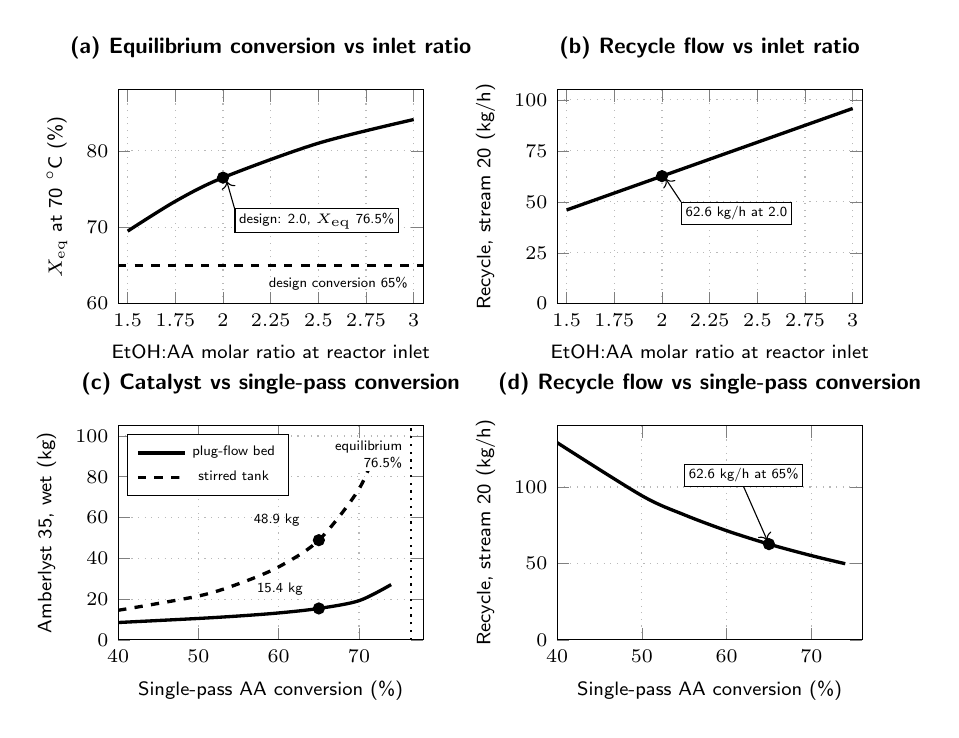
\begin{tikzpicture}
\begin{groupplot}[
    group style={group size=2 by 2, horizontal sep=1.7cm, vertical sep=1.55cm},
    width=0.45\textwidth,
    height=4.3cm,
    grid=both,
    grid style={dotted, gray!55},
    axis lines=box,
    tick label style={font=\sffamily\scriptsize},
    label style={font=\sffamily\scriptsize},
    title style={font=\sffamily\footnotesize\bfseries, at={(0.5,1.02)}, anchor=south}
]

% (a) Equilibrium conversion vs inlet ratio
\nextgroupplot[
    title={(a) Equilibrium conversion vs inlet ratio},
    xlabel={EtOH:AA molar ratio at reactor inlet},
    ylabel={$X_{\mathrm{eq}}$ at 70 $^\circ$C (\%)},
    xmin=1.45, xmax=3.05, ymin=60, ymax=88,
    xtick={1.5,1.75,2.0,2.25,2.5,2.75,3.0},
    ytick={60,70,80}
]
\addplot[solid, very thick, black, smooth] coordinates {
    (1.50,69.5) (1.75,73.4) (2.00,76.5) (2.50,81.0) (3.00,84.1)
};
\addplot[dashed, thick, black, domain=1.45:3.05] {65};
\addplot[only marks, mark=*, mark size=2pt, black] coordinates {(2.00,76.5)};
\node[font=\sffamily\tiny, anchor=north east] at (axis cs:3.02,64.7) {design conversion 65\%};
\node[font=\sffamily\tiny, anchor=north west, draw=black, fill=white, inner sep=1.5pt] (pa) at (axis cs:2.06,72.5) {design: 2.0, $X_{\mathrm{eq}}$ 76.5\%};
\draw[->, black] (pa.north west) -- (axis cs:2.02,76.0);

% (b) Recycle flow vs inlet ratio
\nextgroupplot[
    title={(b) Recycle flow vs inlet ratio},
    xlabel={EtOH:AA molar ratio at reactor inlet},
    ylabel={Recycle, stream 20 (kg/h)},
    xmin=1.45, xmax=3.05, ymin=0, ymax=105,
    xtick={1.5,1.75,2.0,2.25,2.5,2.75,3.0},
    ytick={0,25,50,75,100}
]
\addplot[solid, very thick, black, smooth] coordinates {
    (1.50,46.0) (1.75,54.3) (2.00,62.6) (2.50,79.2) (3.00,95.8)
};
\addplot[only marks, mark=*, mark size=2pt, black] coordinates {(2.00,62.6)};
\node[font=\sffamily\tiny, anchor=north west, draw=black, fill=white, inner sep=1.5pt] (pb) at (axis cs:2.10,50) {62.6~kg/h at 2.0};
\draw[->, black] (pb.north west) -- (axis cs:2.02,61.2);

% (c) Catalyst vs single-pass conversion
\nextgroupplot[
    title={(c) Catalyst vs single-pass conversion},
    xlabel={Single-pass AA conversion (\%)},
    ylabel={Amberlyst 35, wet (kg)},
    xmin=40, xmax=78, ymin=0, ymax=105,
    xtick={40,50,60,70},
    ytick={0,20,40,60,80,100},
    legend style={at={(0.03,0.96)}, anchor=north west, draw=black, fill=white, font=\sffamily\tiny}
]
\addplot[solid, very thick, black, smooth] coordinates {
    (40,8.5) (50,10.5) (55,11.7) (60,13.2) (65,15.4) (70,19.2) (74,27.1)
};
\addlegendentry{plug-flow bed}
\addplot[dashed, very thick, black, smooth] coordinates {
    (40,14.5) (50,21.5) (55,27.5) (60,35.8) (65,48.9) (70,74.0) (72.5,97.0)
};
\addlegendentry{stirred tank}
\draw[dotted, thick, black] (axis cs:76.5,0) -- (axis cs:76.5,105);
\node[font=\sffamily\tiny, align=right, anchor=north east, fill=white, inner sep=1pt] at (axis cs:75.8,99) {equilibrium\\76.5\%};
\addplot[only marks, mark=*, mark size=2pt, black] coordinates {(65,15.4) (65,48.9)};
\node[font=\sffamily\tiny, anchor=south east] at (axis cs:64.2,17) {15.4~kg};
\node[font=\sffamily\tiny, anchor=south east] at (axis cs:63.8,51) {48.9~kg};

% (d) Recycle flow vs single-pass conversion
\nextgroupplot[
    title={(d) Recycle flow vs single-pass conversion},
    xlabel={Single-pass AA conversion (\%)},
    ylabel={Recycle, stream 20 (kg/h)},
    xmin=40, xmax=76, ymin=0, ymax=140,
    xtick={40,50,60,70},
    ytick={0,50,100}
]
\addplot[solid, very thick, black, smooth] coordinates {
    (40,129.0) (50,94.3) (55,81.8) (60,71.4) (65,62.6) (70,55.1) (74,49.8)
};
\addplot[only marks, mark=*, mark size=2pt, black] coordinates {(65,62.6)};
\node[font=\sffamily\tiny, anchor=south west, draw=black, fill=white, inner sep=1.5pt] (pd) at (axis cs:55,100) {62.6~kg/h at 65\%};
\draw[->, black] (pd.south) -- (axis cs:64.8,65);

\end{groupplot}
\end{tikzpicture}
\caption{Reactor design trade-offs at 70~$^\circ$C, with the recycled water and ester included: (a,~b)~effect of the reactor-inlet EtOH:AA ratio at 65\% conversion; (c,~d)~effect of the single-pass conversion at $\mathrm{EtOH:AA} = 2.0$. $K$ and the kinetics from Lai et~al.~\cite{ref7}.}
\label{fig:tradeoffs}
\end{figure}

\begin{table}[H]
\centering
\caption{Sensitivity of the design to the separator recoveries.}
\label{tab:sens}
\small
\begin{tabularx}{\textwidth}{|Y|R{1.7cm}|R{1.4cm}|R{1.4cm}|R{1.4cm}|R{1.8cm}|}
\hline
\hdrrow
\textbf{Case} & \textbf{Fresh feed (kg/h)} & \textbf{Recycle (kg/h)} & \textbf{Catalyst (kg)} & \textbf{Heater (kW)} & \textbf{COD (kg~O$_2$/h)} \\
\hline
Base case: 65\% conversion, 90\% acid and 99\% ethanol recovery & 52.18 & 62.6 & 15.4 & 3.16 & 2.58 \\
\hline
Acid recovery 50\% & 58.30 & 56.5 & 15.4 & 3.20 & 9.10 \\
\hline
Acid recovery 99\% & 50.80 & 64.0 & 15.4 & 3.15 & 1.11 \\
\hline
Ethanol recovery 95\% & 53.99 & 60.8 & 15.4 & 3.17 & 6.35 \\
\hline
Ethanol recovery 99.9\% & 51.77 & 63.0 & 15.4 & 3.16 & 1.73 \\
\hline
\end{tabularx}
\tabnote{Catalyst: wet Amberlyst~35 for plug flow at 70~$^\circ$C.}
\end{table}

\subsection{Equipment and Indicative Economics}
\label{sec:equip_econ}

Table~\ref{tab:equip} gives a preliminary size or duty for each item. The most important number is the last one: the reaction section handles 6.7~kW, but separating the product to specification needs an estimated 23--46~kW, which the component separators cannot represent. Table~\ref{tab:econ} uses European price indices~\cite{ref18}, a mid-market exchange rate~\cite{ref19} and UK non-domestic energy prices~\cite{ref20}, and includes no capital cost.

\begin{table}[H]
\centering
\caption{Preliminary equipment and utility summary.}
\label{tab:equip}
\small
\begin{tabularx}{\textwidth}{|C{2.8cm}|C{4.2cm}|Y|}
\hline
\hdrrow
\textbf{Item} & \textbf{Size or duty} & \textbf{Basis and notes} \\
\hline
RCONV-1 & Fixed bed $0.20\text{ m} \times 1.0\text{ m}$, 25~kg Amberlyst~35 (wet) & Heat removal 0.68~kW (design 1~kW) or adiabatic with a 62~$^\circ$C feed; 316L stainless steel \\
\hline
PUMP-1 & 132~L/h against 1.49~bar; shaft 7.3~W & Metering pump, motor about 0.25~kW; NPSH available about 11~m \\
\hline
HT-1 & 3.16~kW, 0.087~m$^2$ & Steam at 1.2~bar(a) (104.8~$^\circ$C), 5.1~kg/h; wall 5.2~K below the feed's bubble point, so no boiling \\
\hline
CL-1 & 2.84~kW, 0.22~m$^2$ & Cooling water 20 to 30~$^\circ$C, 245~kg/h \\
\hline
Feed--effluent exchanger & 2.32~kW, 0.89~m$^2$ & Optional (Section~\ref{sec:heat_int}) \\
\hline
V-1 & 22~L vertical drum, $0.24\text{ m} \times 0.48\text{ m}$ & Surge and knock-out drum: 5~min hold-up at half level; vent to a safe location \\
\hline
Separation train & About 23--46~kW of reboiler heat & Assumed 2--4~GJ per tonne of EA~\cite{ref16}; the condensers reject about the same heat \\
\hline
\end{tabularx}
\tabnote{Heat-transfer coefficients are mid-range values for steam/organic (0.7), organic/water (0.5) and organic/organic (0.25~kW/(m$^2$\,K)) duties~\cite{ref17}.}
\end{table}

\begin{table}[H]
\centering
\caption{Indicative annual economics (330~days/year).}
\label{tab:econ}
\small
\begin{tabularx}{\textwidth}{|Y|C{3.9cm}|C{2.6cm}|C{3.2cm}|}
\hline
\hdrrow
\textbf{Item} & \textbf{Price} & \textbf{Quantity per year} & \textbf{\pounds\ per year} \\
\hline
Ethyl acetate (product) & US\$1.37/kg = \pounds 1.002/kg & 330.1~t & 330,843 \\
\hline
Acetic acid (fresh) & US\$0.67/kg = \pounds 0.490/kg & 237.1~t & $-116{,}192$ \\
\hline
Ethanol (fresh) & US\$1.07/kg = \pounds 0.783/kg & 176.2~t & $-137{,}908$ \\
\hline
\hdrrow
\textbf{Gross margin (materials)} & & & \textbf{76,743} \\
\hline
Steam, HT-1 (unintegrated) & \pounds 0.062/kWh of heat & 25.0~MWh & $-1{,}555$ \\
\hline
Electricity, pump motor & \pounds 0.245/kWh & 2.0~MWh & $-485$ \\
\hline
Cooling water, CL-1 & \pounds 0.05/m$^3$ (assumed) & 1,938~m$^3$ & $-97$ \\
\hline
Steam, separation & \pounds 0.062/kWh of heat & 183--367~MWh & $-11{,}392$ to $-22{,}785$ \\
\hline
Cooling water, condensers & \pounds 0.05/m$^3$ (assumed) & 15,795--31,590~m$^3$ & $-790$ to $-1{,}580$ \\
\hline
\hdrrow
\textbf{Margin after utilities} & & & \textbf{50,241 to 62,423} \\
\hline
\end{tabularx}
\tabnote{Steam cost = gas price / 85\% boiler efficiency. The pump is charged at the full 0.25~kW motor rating rather than its 7.3~W shaft power, a conservative upper bound. Condenser cooling water assumes the condensers reject the reboiler heat, with a 10~K rise.}
\end{table}

Raw materials cost \pounds 0.77 per kg of EA against a selling price of about \pounds 1.00/kg, leaving roughly \pounds 77k a year before utilities and \pounds 50--62k after them. That would not pay for one operator per shift, before catalyst, maintenance, effluent treatment and capital, so at 330~t/year the plant is a learning-scale basis, not a business. Because materials are about three-quarters of the product value, viability at scale depends on keeping acid and ethanol losses low.

% ==================== SECTION 8 ====================
\section{Safety, Health and Environment}

Table~\ref{tab:pure_comp} lists the physical and hazard properties. Ethyl acetate governs the fire and explosion hazard because its flash point ($-4~^\circ$C) and lower flammable limit (2.0~vol\% in air~\cite{ref4}) allow ignitable vapours at ambient temperature; storage, product transfer and separation therefore require hazardous-area classification, suitable electrical equipment, and earthing and bonding under the UK Dangerous Substances and Explosive Atmospheres Regulations (DSEAR). Acetic acid governs the occupational health and corrosion hazard: its UK Workplace Exposure Limit (WEL) is 10~ppm (8-hour time-weighted average) and 20~ppm (15-minute short-term limit)~\cite{ref6}, and it is strongly corrosive, requiring 316L stainless steel wetted parts and exposure controls under the Control of Substances Hazardous to Health (COSHH) regulations. Under GB mandatory hazard classification~\cite{ref21,ref22}, ethanol carries H225 (highly flammable liquid and vapour); acetic acid carries H226 (flammable liquid) and H314 (severe skin burns and eye damage); and ethyl acetate carries H225, H319 (serious eye irritation) and H336 (drowsiness or dizziness). In addition, glacial acetic acid freezes at 16.6~$^\circ$C~\cite{ref5}---above typical UK ambient temperatures for most of the year---so its storage tank and feed line require insulation, heat tracing and temperature control. Table~\ref{tab:hazop} summarises the screening HAZOP-style review.

\begin{table}[H]
\centering
\caption{Screening HAZOP-style review (not a full HAZOP).}
\label{tab:hazop}
\small
\begin{tabularx}{\textwidth}{|L{2.7cm}|L{2.9cm}|L{3.2cm}|Y|}
\hline
\hdrrow
\textbf{Node} & \textbf{Deviation} & \textbf{Consequence} & \textbf{Safeguards to consider} \\
\hline
Fresh acetic acid storage and feed line & Low temperature (below 16.6~$^\circ$C) & Solidification and line blockage; loss of feed & Insulated, heat-traced lines; storage held at 20--25~$^\circ$C; low-temperature alarm \\
\hline
Feed and recycle tanks & Vapour release, ignition & Fire, exposure above the WEL & Closed transfer, nitrogen blanket, earthing, area classification \\
\hline
PUMP-1 & No flow or blocked outlet & Overheating, seal leak & Low-flow trip, relief to suction, double mechanical seal \\
\hline
HT-1 & High temperature & Boiling in the bed, pressure rise & Steam at 1.2~bar(a), below the feed bubble point; temperature trip \\
\hline
RCONV-1 & High temperature or pressure & Vapour in the bed, release & Pressure relief sized for the fire case, high-temperature alarm \\
\hline
CL-1 & Loss of cooling water & Hot liquid flashing at V-1 & Low-flow alarm on the cooling water; V-1 vent to a safe location \\
\hline
CS-1 (product) & Off-specification product & Customer rejection & Online water and ethanol analysis; recycle of off-specification material \\
\hline
CS-2 and effluent & High acid or ethanol in the effluent & Consent breach, lost material & COD monitoring; acid-recovery performance check \\
\hline
\end{tabularx}
\end{table}

\textbf{Effluent.} Stream~12 is 10.50~kg/h of 81~wt\% water carrying 14.6~wt\% acetic acid, 4.3~wt\% ethanol and a trace of ester. Its chemical oxygen demand (COD) is estimated as the theoretical oxygen demand, the oxygen needed to oxidise each organic completely to $\mathrm{CO_2}$ and water:
\begin{equation}
\mathrm{COD} = \sum_i \dot{m}_i\,\theta_i, \qquad
\theta_{\mathrm{EtOH}} = \frac{3 \times 32}{46.07} = 2.08, \quad
\theta_{\mathrm{AA}} = \frac{2 \times 32}{60.05} = 1.07, \quad
\theta_{\mathrm{EA}} = \frac{5 \times 32}{88.11} = 1.82
\label{eq:cod}
\end{equation}
where $\dot{m}_i$ is the mass flow of component $i$ in the waste and $\theta_i$ is in kg~O$_2$ per kg, from $\mathrm{C_2H_5OH + 3\,O_2 \to 2\,CO_2 + 3\,H_2O}$, $\mathrm{CH_3COOH + 2\,O_2 \to 2\,CO_2 + 2\,H_2O}$ and $\mathrm{C_4H_8O_2 + 5\,O_2 \to 4\,CO_2 + 4\,H_2O}$. The result, 2.58~kg~O$_2$/h or about 243~g/L, is far too concentrated for direct discharge. The components are readily biodegradable, so neutralisation and biological treatment under a trade-effluent consent is a realistic route, and better acid recovery would cut the load (Table~\ref{tab:sens}).

% ==================== SECTION 9 ====================
\section{Conclusions, Limitations and Next Steps}

\subsection{Main Findings}
\begin{itemize}
    \item \textbf{Both DWSIM runs reproduce the hand calculation.} Every component flow agrees within 0.009\% and all twelve acceptance checks pass in each run. The product, 41.68~kg/h at 99.96~wt\% EA, meets the composition limits of the specification.
    \item \textbf{The 65\% basis is feasible only because of the ethanol excess.} At $\mathrm{EtOH:AA} = 2.0$, model-dependent equilibrium estimates give 73.5--81.2\%, whereas an equimolar feed yields only 62--67\%. A plug-flow bed needs 15.4~kg of catalyst against 48.9~kg in a stirred tank.
    \item \textbf{Convergence is not proof.} A Python reconstruction of DWSIM's default recycle tolerance predicts premature termination at 41\% of the true recycle flow, at an inlet ratio where 65\% conversion exceeds the model-estimated equilibrium limit; with a tightened tolerance ($1 \times 10^{-8}$~kg/s), the solved recycle sits within 0.006\% of the exact steady state.
    \item \textbf{Enthalpy selection strongly affects predicted duties.} Lee--Kesler predicts heater and cooler duties 16--19\% above the ideal-liquid benchmark; Liquid $C_p$ agrees closely with the independent ideal-liquid benchmark (requiring further comparison with excess-enthalpy data to establish full physical accuracy) while reporting a reactor duty 1.75~kW higher, consistent with an ideal-gas reaction-enthalpy reference offset.
    \item \textbf{The NRTL database needs auditing.} Two pairs are estimated from UNIFAC, the ternary azeotrope ester mole fraction differs from literature by 0.087 (0.666 vs.\ 0.579), a spurious acetic acid--water azeotrope appears, and the ethyl acetate--water miscibility gap is far too narrow for decanter design.
\end{itemize}

\subsection{Limitations and Next Steps}
\begin{itemize}
    \item \textbf{Separation.} CS-1 and CS-2 meet the specification by construction and carry no energy, although the separation train dominates the plant's energy use. Next: a decanter and rigorous columns, with liquid--liquid NRTL parameters and a flash set to vapour--liquid--liquid.
    \item \textbf{Thermodynamics.} The vapour is ideal, so acetic acid dimerisation is ignored. Next: a vapour model with dimerisation for the acid-recovery column.
    \item \textbf{Reaction.} The 65\% conversion is imposed, and the kinetics come from one laboratory study over 60--80~$^\circ$C, with catalyst ageing covered only by the 25\% margin. Next: a kinetic plug-flow reactor using the rate law of Section~\ref{sec:kinetics}, cross-checked against the activity-based model of Calvar et~al.~\cite{ref23}.
    \item \textbf{Heat integration and economics.} The feed--effluent exchanger is hand-calculated only, and the economics exclude capital and use one month's prices. Next: add the exchanger to the DWSIM model and estimate capital cost.
\end{itemize}

% ==================== NOMENCLATURE ====================
\clearpage
\section*{Nomenclature}
\addcontentsline{toc}{section}{Nomenclature}

\begin{table}[H]
\centering
\scriptsize
\renewcommand{\arraystretch}{1.12}
\setlength{\tabcolsep}{4pt}
\begin{tabularx}{\textwidth}{|C{3.3cm}|Z|C{4.3cm}|}
\hline
\hdrrow
\textbf{Symbol / Term} & \textbf{Meaning} & \textbf{Units} \\
\hline
$A_{ij}$ & NRTL binary interaction energy parameter & cal/mol \\
\hline
$a_i$ & Liquid-phase thermodynamic activity of component $i$ & dimensionless \\
\hline
$C_i$ & Liquid molar concentration of component $i$ & mol/cm$^3$ \\
\hline
$C_p$ & Liquid isobaric molar heat capacity & kJ/(kmol\,K) \\
\hline
E1--E6 & Flowsheet equipment energy stream duties & kW (E1 also W) \\
\hline
$E_{a,1}$, $E_{a,-1}$ & Forward and reverse reaction activation energies & J/mol \\
\hline
$F_{\mathrm{AA},0}$ & Reactor-inlet molar flow rate of acetic acid & mol/min \\
\hline
$G_{ij}$ & NRTL Boltzmann weighting factor, $\exp(-\alpha_{ij}\tau_{ij})$ & dimensionless \\
\hline
$g_i$ & Recycle loop gain of component $i$, $(1-s_i)r_i$ & dimensionless \\
\hline
$\Delta_{\mathrm{f}}H^\circ$, $\Delta_{\mathrm{r}}H^\circ$ & Standard enthalpy of formation and reaction & kJ/mol \\
\hline
$\Delta_{\mathrm{r}}H_{\mathrm{l}}$, $\Delta_{\mathrm{r}}H_{\mathrm{ig}}$ & Liquid-phase and ideal-gas enthalpy of reaction & kJ/mol (or kJ/kmol) \\
\hline
$\Delta H_{\mathrm{vap}}$ & Enthalpy of vaporisation & kJ/mol \\
\hline
$K$, $K_x$ & Mole-fraction chemical equilibrium constant & dimensionless \\
\hline
$K_a$ & Thermodynamic activity equilibrium constant & dimensionless \\
\hline
$k_1$, $k_{-1}$ & Forward and reverse kinetic rate constants & cm$^6$\,mol$^{-1}$\,g$^{-1}$\,min$^{-1}$ \\
\hline
$M$ & Pure-component molar mass & kg/kmol \\
\hline
$\dot{m}_i$ & Mass flow rate of component $i$ & kg/h \\
\hline
$P$, $P_i^{\mathrm{sat}}$ & System pressure and saturation vapour pressure & bar \\
\hline
$\Delta P$ & Pressure drop across equipment or catalyst bed & bar (or kPa) \\
\hline
$R$ & Universal gas constant & 8.3145 J/(mol\,K) or 1.98721 cal/(mol\,K) \\
\hline
$r'$ & Catalyst-mass-based reaction rate (wet catalyst basis) & mol\,g$^{-1}$\,min$^{-1}$ \\
\hline
$r_i$, $s_i$ & CS-2 recycle split fraction and CS-1 product split fraction & dimensionless \\
\hline
$T$, $T_{\mathrm{b}}$, $T_{\mathrm{m}}$, $T_{\mathrm{fus}}$ & Operating, normal boiling, melting and fusion temperatures & K or $^\circ$C \\
\hline
$U$ & Overall heat-transfer coefficient & kW/(m$^2$\,K) \\
\hline
$W$, $W_{\mathrm{PFR}}$, $W_{\mathrm{CSTR}}$ & Wet catalyst mass (plug-flow bed and stirred tank) & kg (g inside Eq.~\eqref{eq:pfr}) \\
\hline
$X$, $X_{\mathrm{eq}}$ & Single-pass and equilibrium acetic acid conversion & dimensionless (or \%) \\
\hline
$x_i$ & Liquid-phase mole fraction of component $i$ & dimensionless \\
\hline
$\alpha_{ij}$ & NRTL non-randomness parameter & dimensionless \\
\hline
$\gamma_i$, $\Gamma$ & Liquid activity coefficient and activity-coefficient ratio in Eq.~\eqref{eq:ka} & dimensionless \\
\hline
$\delta$ & Tear-stream mass-flow step on final recycle iteration & kg/s \\
\hline
$\theta_i$ & Theoretical oxygen demand factor of component $i$ & kg~O$_2$/kg \\
\hline
$\nu_i$ & Stoichiometric coefficient of component $i$ & dimensionless \\
\hline
$\xi$ & Molar extent of reaction & kmol/h \\
\hline
$\tau_{ij}$ & Dimensionless NRTL interaction parameter, $A_{ij}/(RT)$ & dimensionless \\
\hline
\multicolumn{3}{|c|}{\textbf{Abbreviations}} \\
\hline
AA, EA, EtOH, W & Acetic acid, ethyl acetate, ethanol, water & -- \\
\hline
BV, LHSV & Bed volumes; liquid hourly space velocity & dimensionless; h$^{-1}$ (BV/h) \\
\hline
COD & Chemical oxygen demand & kg~O$_2$/h (or g/L) \\
\hline
COSHH, DSEAR & UK Control of Substances Hazardous to Health; Dangerous Substances and Explosive Atmospheres Regulations & -- \\
\hline
CSTR, PFR & Continuous stirred-tank reactor; plug-flow reactor & -- \\
\hline
HAZOP & Hazard and operability study & -- \\
\hline
NPSH & Net positive suction head & m \\
\hline
NRTL, UNIFAC & Non-Random Two-Liquid; Universal Quasichemical Functional-group Activity Coefficients & -- \\
\hline
VLE, LLE, VLLE & Vapour--liquid, liquid--liquid and vapour--liquid--liquid equilibrium & -- \\
\hline
WEL & UK Workplace Exposure Limit (8-h TWA / 15-min STEL) & ppm \\
\hline
\end{tabularx}
\end{table}
\clearpage

% ==================== REFERENCES ====================
\begingroup
\footnotesize
\justifying
\sloppy
\begin{thebibliography}{23}
\addcontentsline{toc}{section}{References}
\setlength{\itemsep}{2pt}

\bibitem{ref1} BP starts commercial production from world's largest ethyl acetate plant (220,000~t/year, Avada process, Saltend, Hull). \textit{chemeurope.com}, 4 December 2001. \url{https://www.chemeurope.com/en/news/6403/bp-starts-commercial-production-from-world-s-largest-ethyl-acetate-plant.html}. (Accessed November 2026.)

\bibitem{ref2} UK: INEOS suspends production at three Hull acetyls plants. \textit{HazardEx}, 29 September 2026. \url{https://www.hazardexonthenet.net/article/224252/UK-INEOS-suspends-production-at-three-Hull-acetyls-plants.aspx}.

\bibitem{ref3} SIPCHEM. Ethyl acetate product specifications (with ASTM test methods), 2023. \url{https://sipchem.is.sa/sites/default/files/2023-10/Ethyl%20Acetate%20Product%20Specifications_0.pdf}.

\bibitem{ref4} National Institute for Occupational Safety and Health. \textit{NIOSH Pocket Guide to Chemical Hazards}: ethyl acetate, acetic acid and ethyl alcohol. \url{https://www.cdc.gov/niosh/npg/npgd0260.html}, \url{https://www.cdc.gov/niosh/npg/npgd0002.html} and \url{https://www.cdc.gov/niosh/npg/npgd0262.html}.

\bibitem{ref5} National Institute of Standards and Technology. Condensed phase thermochemistry data for ethanol (Chao and Rossini, 1965), acetic acid (Steele et~al., 1997), ethyl acetate (Wiberg and Waldron, 1991) and water (CODATA, Cox et~al., 1984); liquid heat capacities; phase-change data for acetic acid ($T_{\mathrm{fus}} = 289.6$~K). In P.~J.~Linstrom and W.~G.~Mallard, editors, \textit{NIST Chemistry WebBook}, NIST Standard Reference Database Number~69. \url{https://webbook.nist.gov}.

\bibitem{ref6} Health and Safety Executive. \textit{EH40/2005 Workplace Exposure Limits}. HSE Books, 4th edition, 2020. \url{https://www.hse.gov.uk/pubns/priced/eh40.pdf}.

\bibitem{ref7} I.-K.~Lai, Y.-C.~Liu, C.-C.~Yu, M.-J.~Lee, and H.-P.~Huang. Production of high-purity ethyl acetate using reactive distillation: experimental and start-up procedure. \textit{Chemical Engineering and Processing}, 47:1831--1843, 2008.

\bibitem{ref8} DWSIM. Open-source process simulator: source code (GitHub repository \texttt{DanWBR/dwsim}, commit \texttt{1abf72d}, 17 July 2026), \url{https://github.com/DanWBR/dwsim}, and user guide, \url{https://dwsim.org/help/main/25-reactors.html}.

\bibitem{ref9} E.~\.{I}nce. Kinetic of esterification of ethyl alcohol by acetic acid on a catalytic resin. \textit{Pamukkale University Journal of Engineering Sciences}, 8(1):109--113, 2002.

\bibitem{ref10} M.~Berthelot and L.~P\'ean de Saint-Gilles. Recherches sur les affinit\'es. \textit{Annales de Chimie et de Physique}, 1862--1863. The classic two-thirds conversion of an equimolar mixture of acetic acid and ethanol.

\bibitem{ref11} A.~Golikova, A.~Samarov, M.~Trofimova, et~al. Chemical equilibrium for the reacting system acetic acid--ethanol--ethyl acetate--water at 303.15~K, 313.15~K and 323.15~K. \textit{Journal of Solution Chemistry}, 46:374--387, 2017. doi:10.1007/s10953-017-0583-1.

\bibitem{ref12} DuPont (formerly Dow and Rohm and Haas). \textit{Amberlyst\texttrademark\ 35 Wet polymeric catalyst, product data sheet}: shipping weight 800~g/L, maximum operating temperature 150~$^\circ$C, 1--5~BV/h, minimum bed depth 1~m.

\bibitem{ref13} S.~Banerjee. Solubility of organic mixtures in water. \textit{Environmental Science \& Technology}, 18(8):587--591, 1984. Value for ethyl acetate, $8.0 \times 10^4$~mg/L at 25~$^\circ$C, as compiled in PubChem (CID~8857).

\bibitem{ref14} M.~Trofimova, A.~Sadaev, A.~Samarov, A.~Golikova, N.~Tsvetov, M.~Toikka, and A.~Toikka. Liquid--liquid equilibrium of acetic acid--ethanol--ethyl acetate--water quaternary system: data review and new results at 323.15~K and 333.15~K. \textit{Fluid Phase Equilibria}, 503:112321, 2020. doi:10.1016/j.fluid.2019.112321.

\bibitem{ref15} W.~L.~Luyben. Snowball effects in reactor/separator processes with recycle. \textit{Industrial \& Engineering Chemistry Research}, 33(2):299--305, 1994.

\bibitem{ref16} R.~M.~Filipe, P.~Castro, H.~A.~Matos, and A.~Q.~Novais. Analysis of processing systems involving reaction and distillation: the synthesis of ethyl acetate. In \textit{CHEMPOR 2005, 9th International Chemical Engineering Conference}, Coimbra, 2005.

\bibitem{ref17} R.~K.~Sinnott. \textit{Coulson \& Richardson's Chemical Engineering, Volume 6: Chemical Engineering Design}. Elsevier, 4th edition, 2005. Table~12.1, typical overall heat-transfer coefficients.

\bibitem{ref18} businessanalytiq. Price indices for ethyl acetate, acetic acid and ethanol, September 2026 (Europe: US\$1.37, 0.67 and 1.07 per kg). \url{https://businessanalytiq.com/procurementanalytics/index/ethyl-acetate-price-index/}.

\bibitem{ref19} Best Exchange Rates. Mid-market exchange rate, November 2026: US\$1.367 per \pounds 1. \url{https://www.bestexchangerates.com/rates/gbp-to-usd}.

\bibitem{ref20} Department for Energy Security and Net Zero. \textit{Quarterly Energy Prices, September 2026} (Q2~2026 non-domestic gas 5.28~p/kWh and electricity 24.51~p/kWh, including the Climate Change Levy), 2026.

\bibitem{ref21} European Chemicals Agency. Table of harmonised entries in Annex~VI to CLP, Regulation (EC) No~1272/2008: index numbers 603-002-00-5 (ethanol), 607-002-00-6 (acetic acid) and 607-022-00-5 (ethyl acetate). \url{https://echa.europa.eu/information-on-chemicals/annex-vi-to-clp}.

\bibitem{ref22} Health and Safety Executive. The CLP Regulation in Great Britain: all EU harmonised classification and labelling in force on 31~December 2020 became GB mandatory classification and labelling (GB~MCL). \url{https://www.hse.gov.uk/chemical-classification/legal/clp-regulation.htm}.

\bibitem{ref23} N.~Calvar, B.~Gonz\'alez, and A.~Dom\'inguez. Esterification of acetic acid with ethanol: reaction kinetics and operation in a packed bed reactive distillation column. \textit{Chemical Engineering and Processing}, 46:1317--1323, 2007. doi:10.1016/j.cep.2006.10.007.

\end{thebibliography}
\endgroup

% ==================== APPENDIX A ====================
\newpage
\appendix
\section{Reproducibility and DWSIM As-Built Inputs}

Table~\ref{tab:dwsim_inputs} lists the inputs of both solved DWSIM files, as read by the script; every input matches the design basis. Figure~\ref{fig:dwsim_screens} shows the two solved flowsheets.

\begin{table}[H]
\centering
\caption{DWSIM 10.0 inputs, identical in both files except for the enthalpy method.}
\label{tab:dwsim_inputs}
\small
\begin{tabularx}{\textwidth}{|L{4.2cm}|Y|}
\hline
\hdrrow
\textbf{Object} & \textbf{Specification} \\
\hline
Compounds and property package & Ethanol, acetic acid, ethyl acetate, water (ChemSep); NRTL with the parameters of Table~\ref{tab:nrtl}; ideal vapour \\
\hline
Enthalpy method & Case~A: Lee--Kesler (default). Case~B: Liquid $C_p$ + Enthalpy of Vaporization. Nothing else differs \\
\hline
Reaction & Conversion reaction $\mathrm{AA + EtOH \to EA + H_2O}$; base compound acetic acid; 65\%; liquid phase \\
\hline
Fresh Ethanol, Fresh Acetic Acid & Ethanol 22.2459~kg/h and acetic acid 29.9327~kg/h, both at 25~$^\circ$C and 1.01325~bar \\
\hline
MIX-1, MIX-2 & Outlet pressure: the lowest of the inlet pressures in both \\
\hline
PUMP-1 & Pressure increase 1.48675~bar, giving 2.5~bar; 75\% efficiency \\
\hline
HT-1 / RCONV-1 / CL-1 & 70~$^\circ$C, 0.2~bar drop / 70~$^\circ$C (outlet-temperature mode), 0.3~bar drop / 35~$^\circ$C, 0.2~bar drop \\
\hline
VALVE-1 and V-1 & 1.01325~bar outlet; adiabatic flash \\
\hline
CS-1 / CS-2 (\% of inlet to top) & CS-1 to \texttt{Product-EtAc}: EtOH 0.01, AA 0.005, EA 99, water 0.08. CS-2 to \texttt{Recycle-1}: EtOH 99, AA 90, EA 99, water 30 \\
\hline
R-1 recycle & Tear at stream~20; tolerance $1 \times 10^{-8}$~kg/s and 0.01~K; up to 1,000 iterations; no acceleration \\
\hline
\end{tabularx}
\end{table}

\begin{figure}[H]
\centering
\begin{subfigure}{\textwidth}
\centering
\IfFileExists{dwsim_caseA.png}{%
    \fbox{\includegraphics[width=0.96\textwidth]{dwsim_caseA.png}}%
}{%
    \fbox{\parbox[c][3.2cm][c]{0.95\textwidth}{\centering\small\textit{Place DWSIM Case A screenshot here as \texttt{dwsim\_caseA.png} (render in greyscale for strict B\&W).}}}%
}
\caption{Case A, Lee--Kesler: E2 3.67, E3 0.75, E4 3.39, E5 0.28 and E6 0.19~kW.}
\end{subfigure}

\vspace{8pt}

\begin{subfigure}{\textwidth}
\centering
\IfFileExists{dwsim_caseB.png}{%
    \fbox{\includegraphics[width=0.96\textwidth]{dwsim_caseB.png}}%
}{%
    \fbox{\parbox[c][3.2cm][c]{0.95\textwidth}{\centering\small\textit{Place DWSIM Case B screenshot here as \texttt{dwsim\_caseB.png} (render in greyscale for strict B\&W).}}}%
}
\caption{Case B, Liquid $C_p$ + Enthalpy of Vaporization: E2 3.16, E3 2.43, E4 2.84, E5 and E6 0.00~kW.}
\end{subfigure}
\caption{The two flowsheets as solved in DWSIM 10.0. The energy streams show DWSIM's own duties; E1 (7~W) displays as 0.01~kW.}
\label{fig:dwsim_screens}
\end{figure}

\textbf{Files and how to run them.} The project consists of the solved flowsheets \texttt{Ethyl\_Acetate\_CaseA\_LeeKesler.dwxmz} and \texttt{Ethyl\_Acetate\_CaseB\_LiquidCp.dwxmz}; the workbook \texttt{Ethyl\_Acetate\_Two\_Model\_Validation\_Comparison.xlsx}, which sets DWSIM's exports of the two runs side by side; and two Python scripts. \texttt{Ethyl\_Acetate\_Calculations.py} (NumPy and SciPy) solves the hand calculation and validates every \texttt{.dwxmz} file in its folder, without needing DWSIM; its NRTL and UNIFAC routines reproduce the open-source \textit{thermo} library to machine precision. \texttt{make\_figures.py} checks the key numbers and redraws Figures~1--4.

\textbf{AI-Assistance Disclosure.} The DWSIM flowsheets (\texttt{Case A} and \texttt{Case B}), property-package configurations, simulation runs, spreadsheet comparisons and engineering verification checks were built and executed by the author. AI assistants (ChatGPT, Claude and Gemini) were used as supporting tools for technical review, verification-script drafting, document formatting and editorial refinement; all engineering assumptions, equations, simulation inputs and final interpretations were reviewed and verified by the author.

\end{document}
